
\begin{center}
\begin{figure}[h!]
\begin{subfigure}[b]{.45\textwidth}
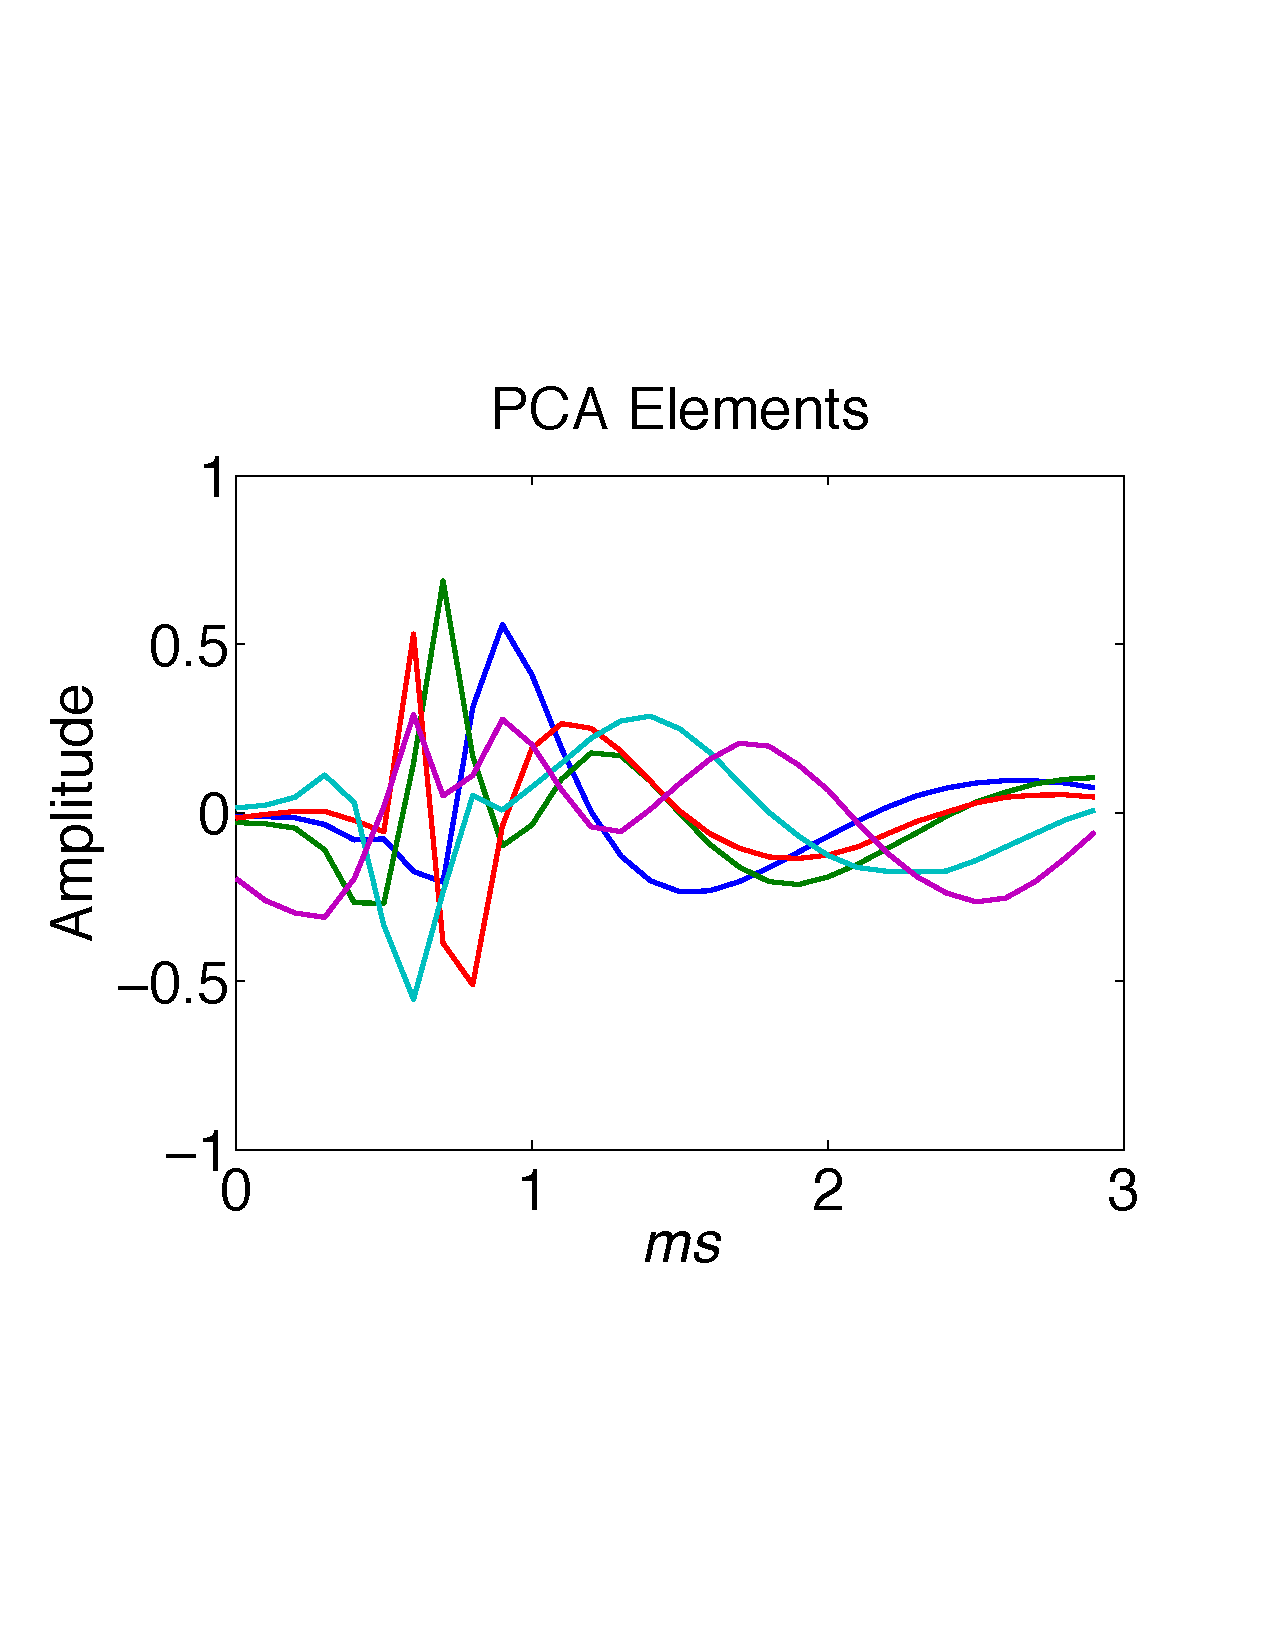
\includegraphics[width=1\textwidth]{../figs/new/pcaelements.pdf}
\caption{}
%\label{fig:ICold}
\end{subfigure}
\begin{subfigure}[b]{.45\textwidth}
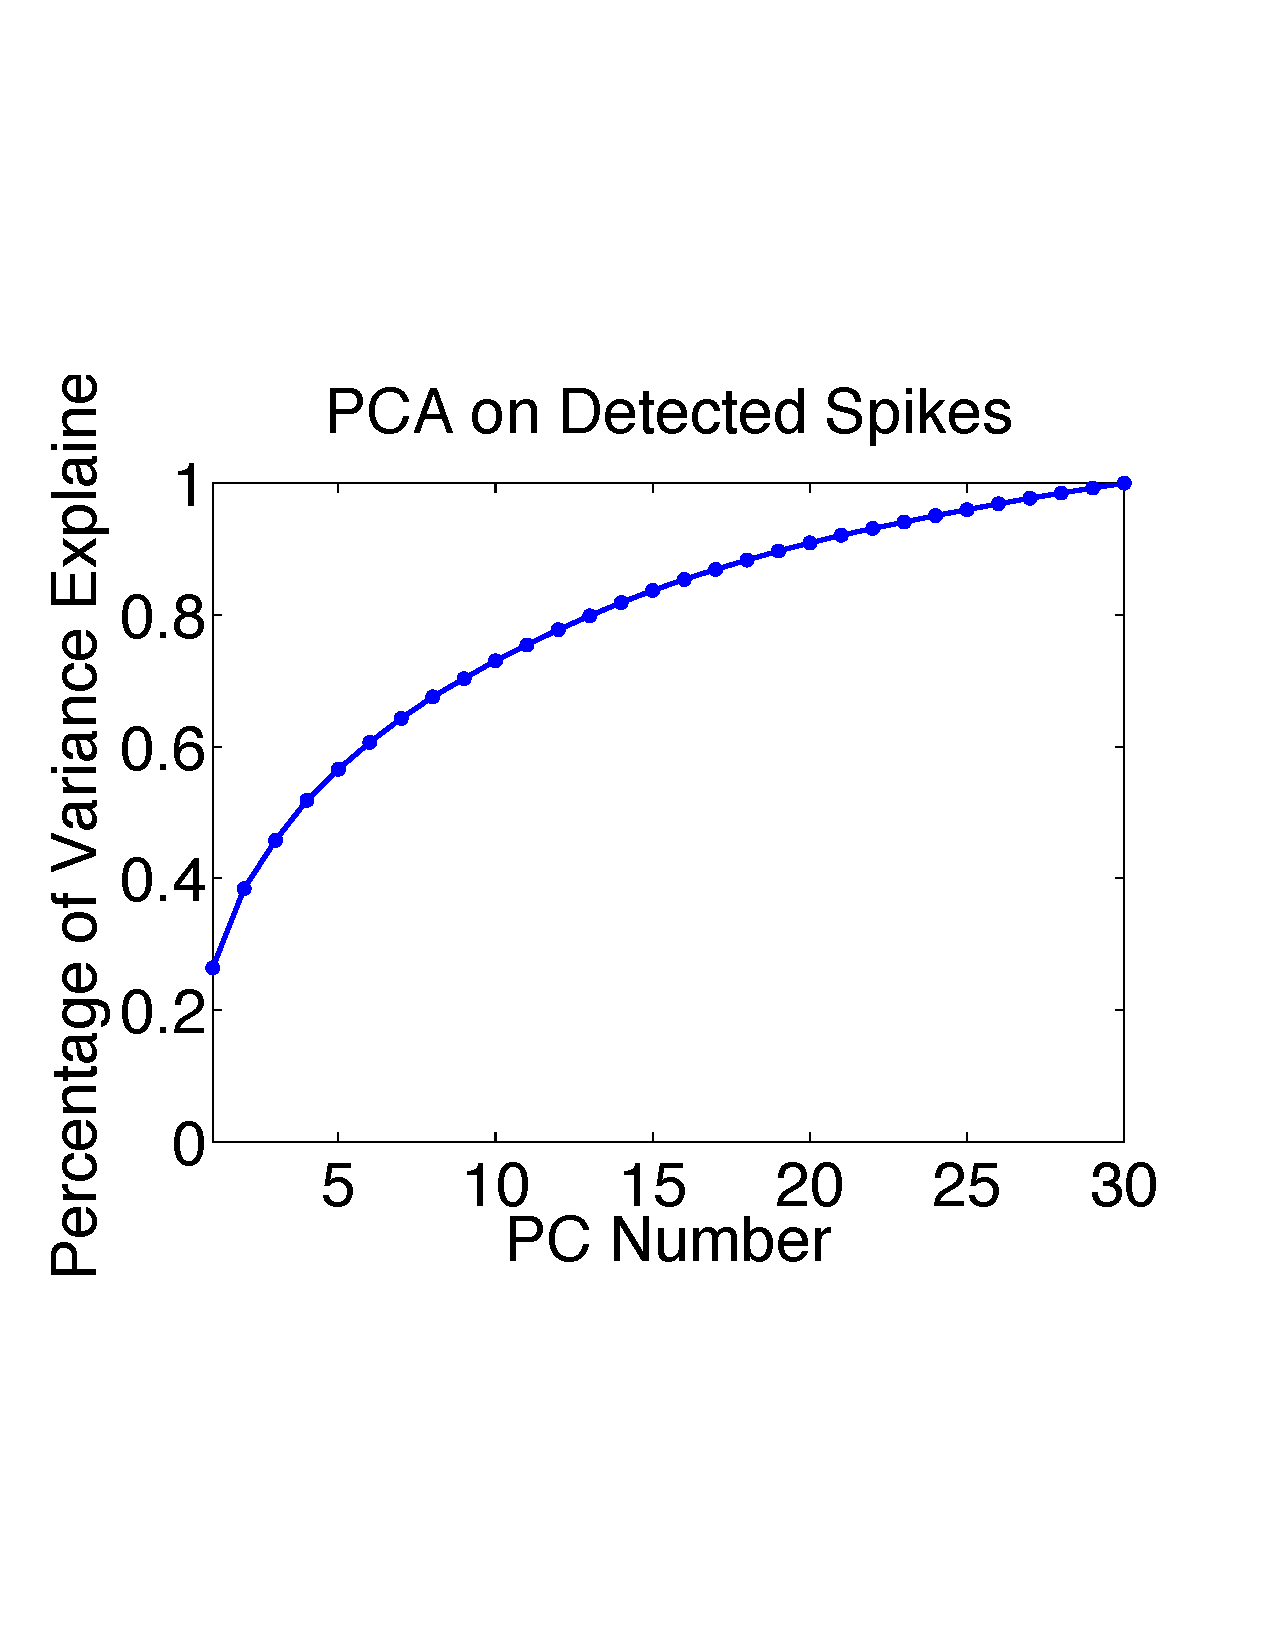
\includegraphics[width=1\textwidth]{../figs/supfigs/pcaenergy.pdf}
\caption{}
\label{fig:PCAenergy}
\end{subfigure}
% \begin{subfigure}[b]{.3\textwidth}
% % 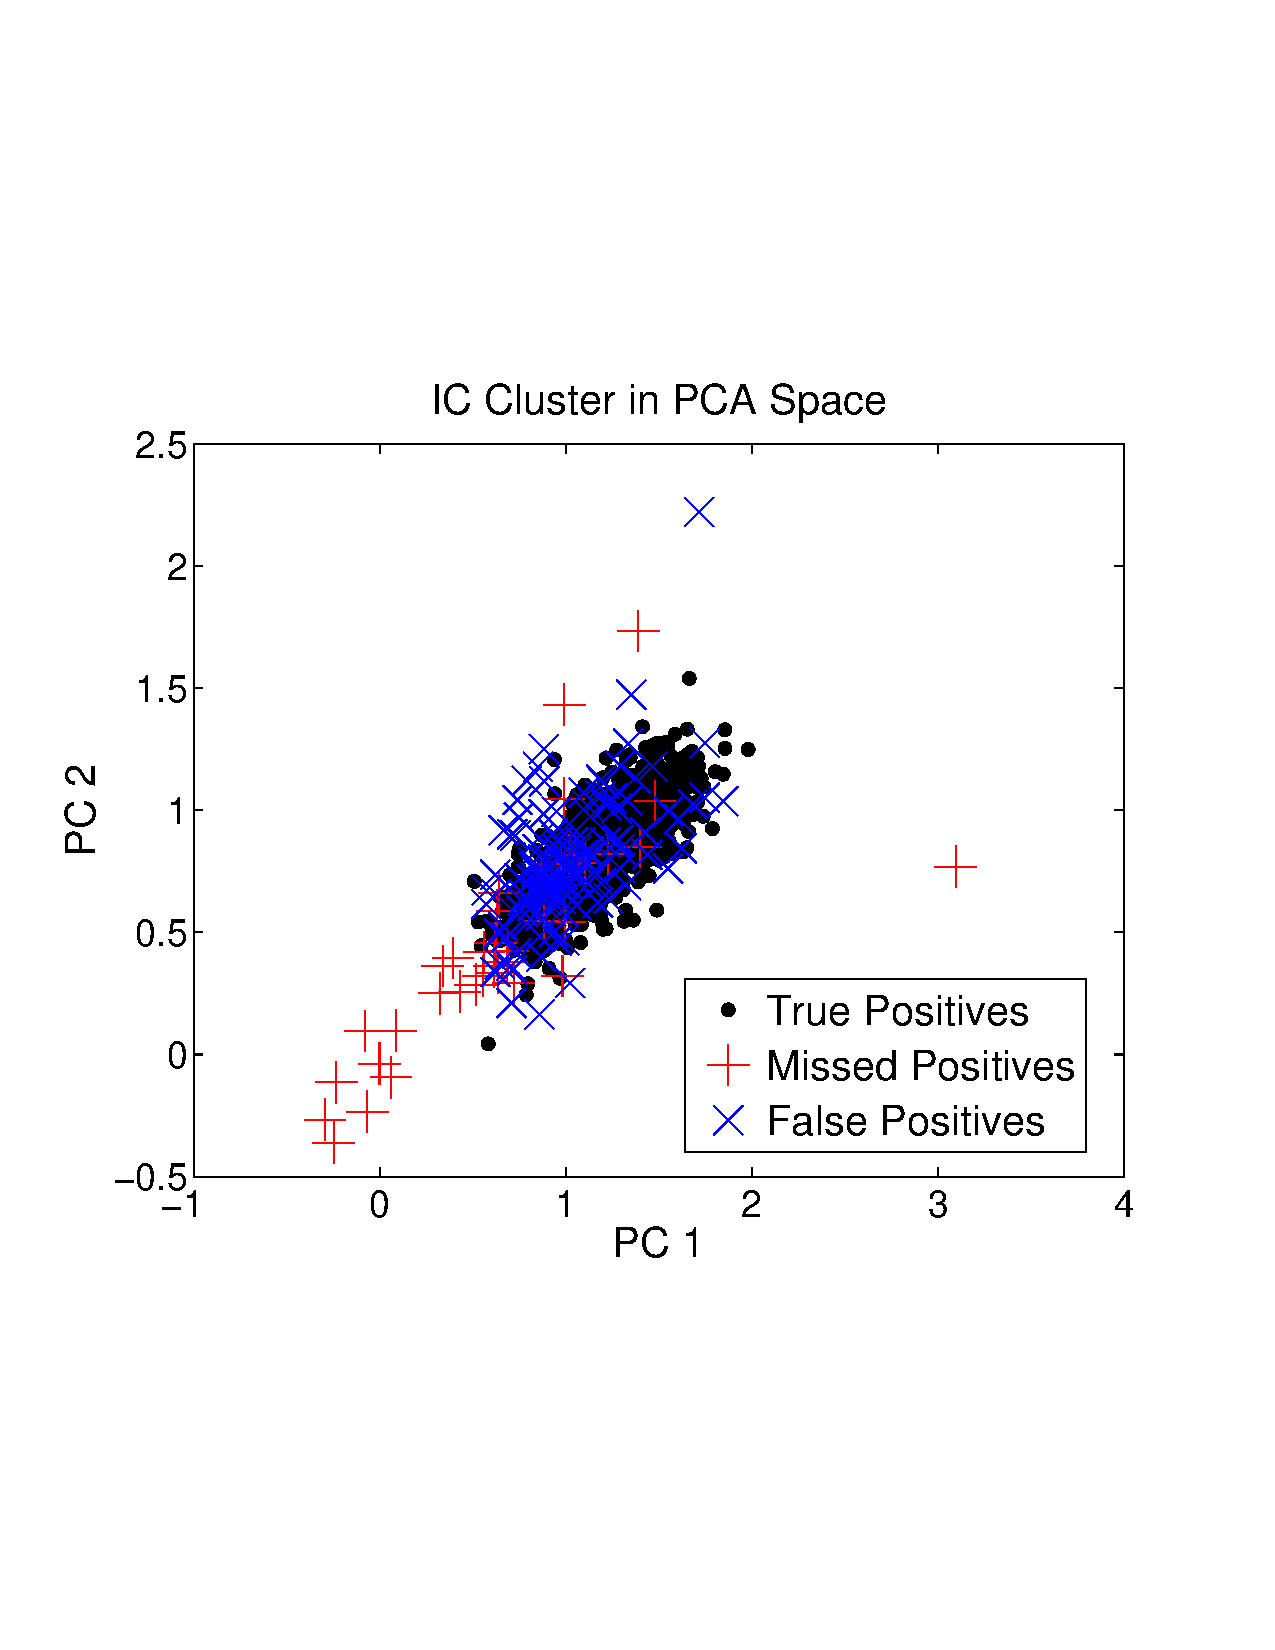
\includegraphics[width=\textwidth]{../figs/new/ICclusteroldpca.pdf}
% \caption{}
% \label{fig:ICold}
% \end{subfigure}
% \begin{subfigure}[b]{.3\textwidth}
% % 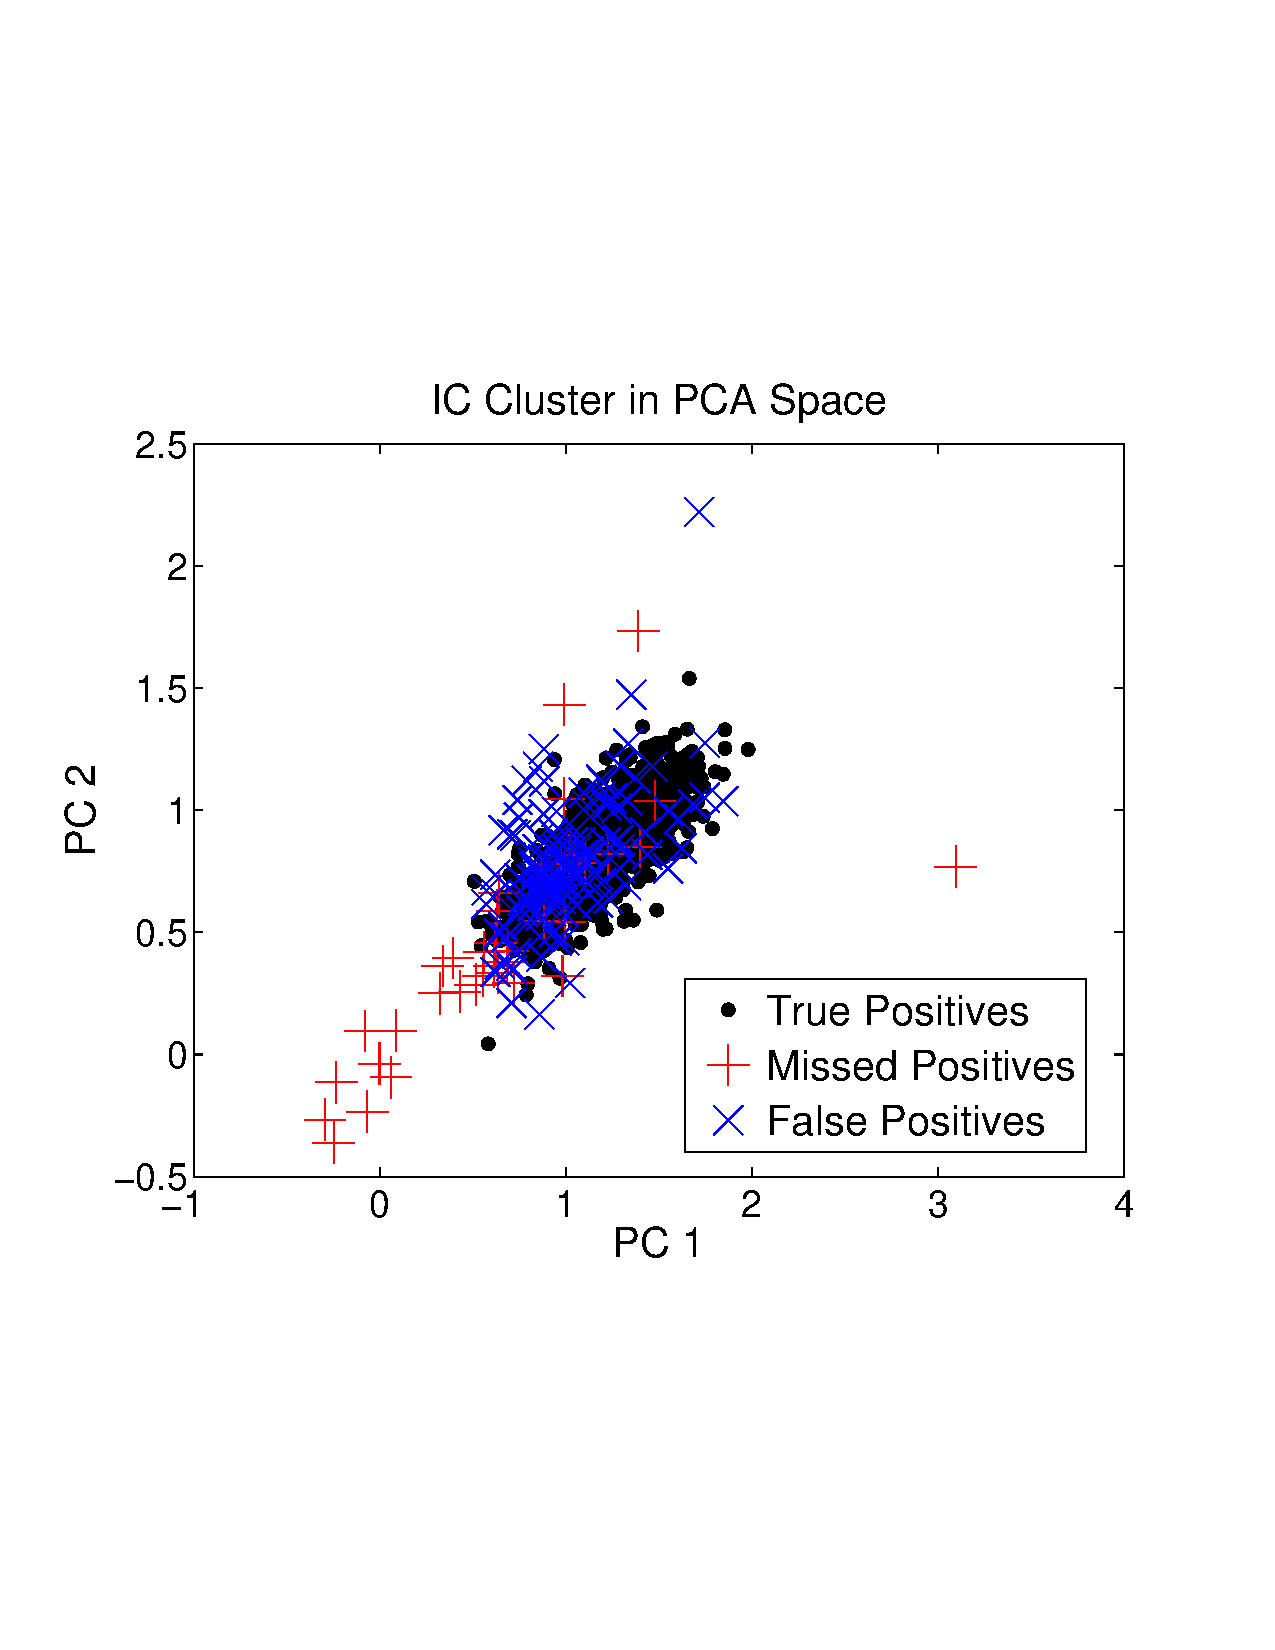
\includegraphics[width=\textwidth]{../figs/new/ICclusteroldpca.pdf}
% \caption{}
% \label{fig:ICold}
% \end{subfigure}
\caption{(a)Dictionary learned from the first 5 seconds of data from the HC1 dataset. (b) Percentage of variance explained by each PCA component.
} \label{fig:dict}
\end{figure}
\end{center}

\begin{figure}[htbp]
	\centering
 	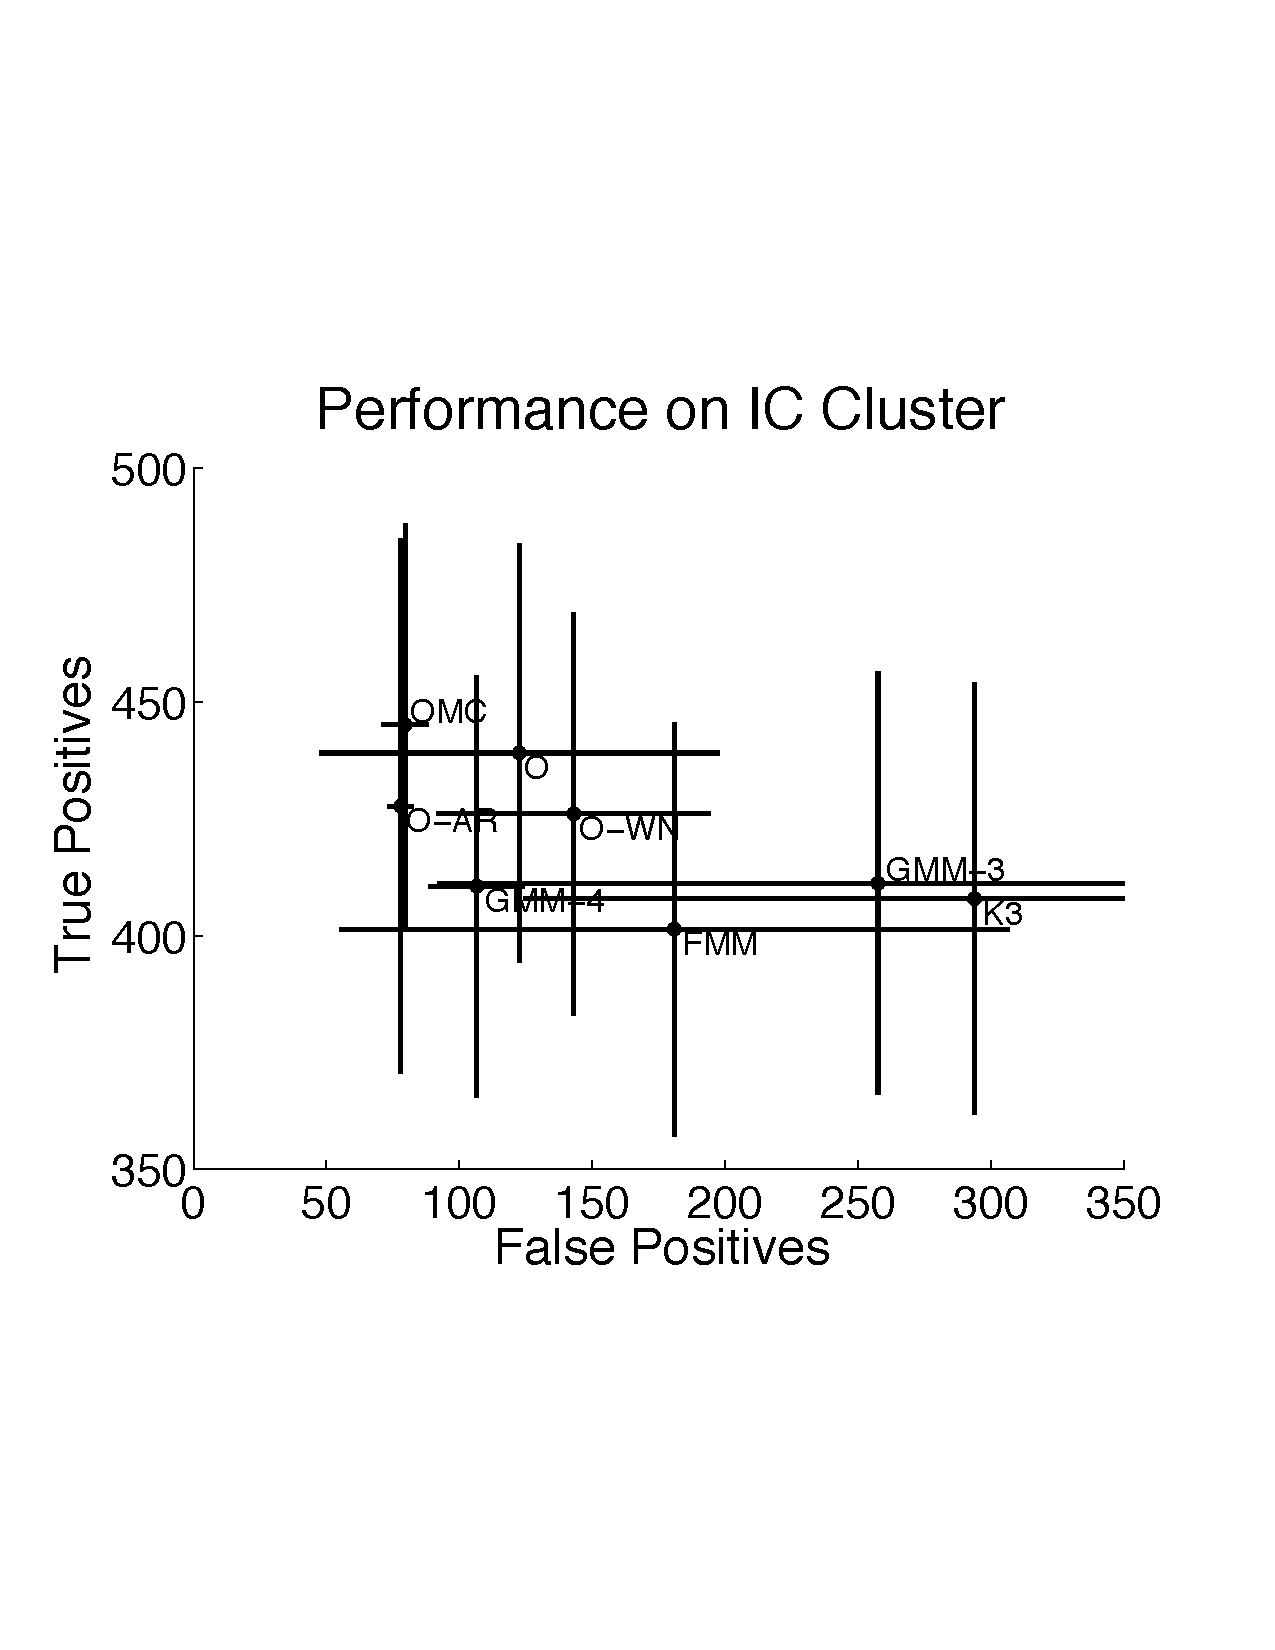
\includegraphics[height=3in]{../figs/supfigs/clusterpermerr.pdf}
	\caption{(a) This shows the average number of true positives versus the average number of false positives in the intracellular cluster for 2 minute segments of the 4 minutes of the experiment.  \smug\ does better than all the competitors.  }
	\label{fig:asdf}
\end{figure}



\begin{center}
\begin{figure}[h!]
\begin{subfigure}[b]{.2\textwidth}
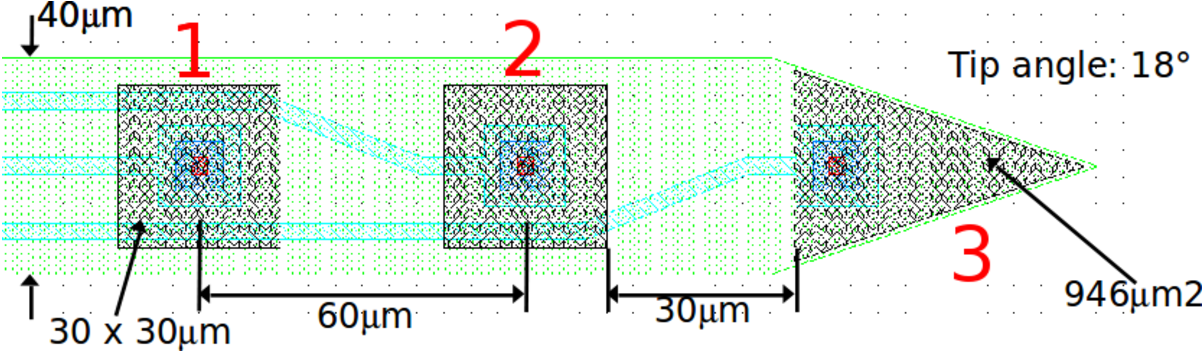
\includegraphics[width=1\textwidth]{../figs/3dev}
\caption{}
\label{3dev}
\end{subfigure}
% \begin{subfigure}[b]{.28\textwidth}
% 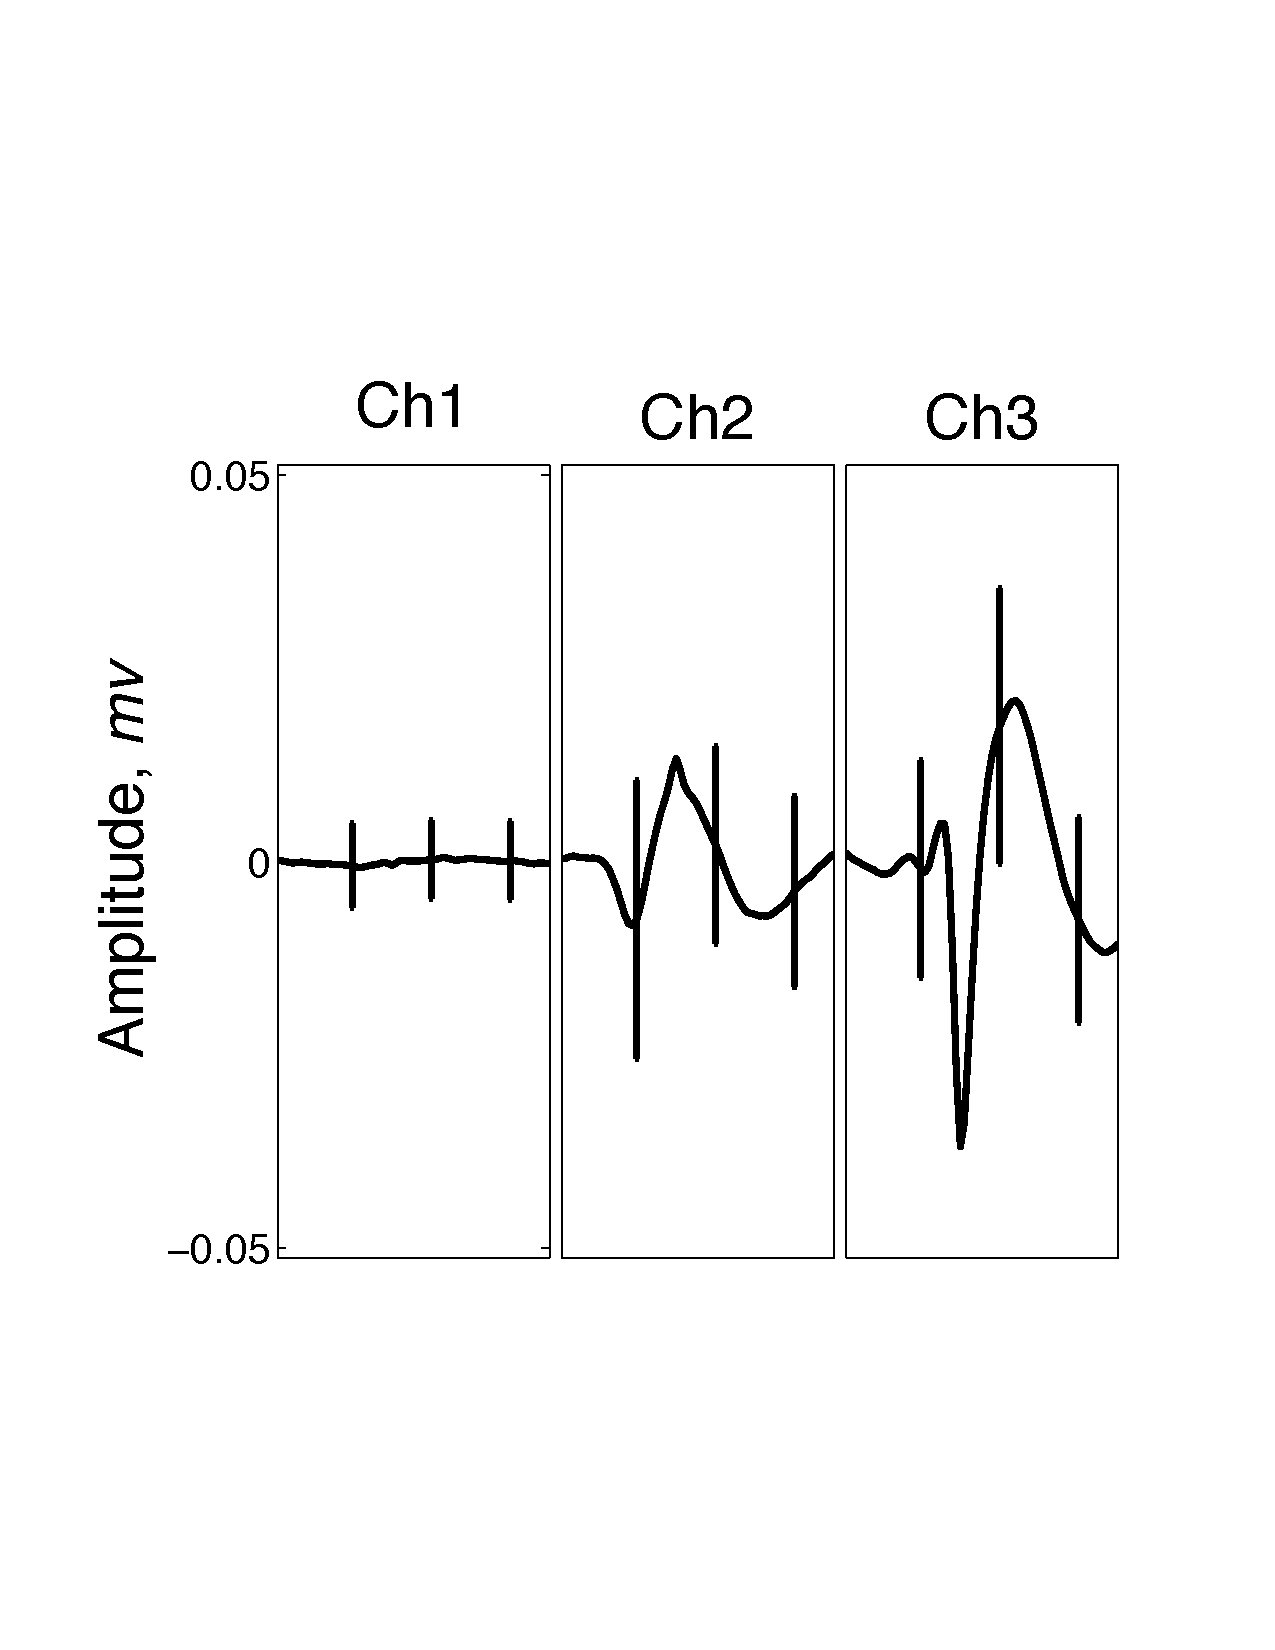
\includegraphics[width=\textwidth]{../figs/3devim/clus1}
% \caption{}
% \label{ex31}
% \end{subfigure}
% \begin{subfigure}[b]{.28\textwidth}
% 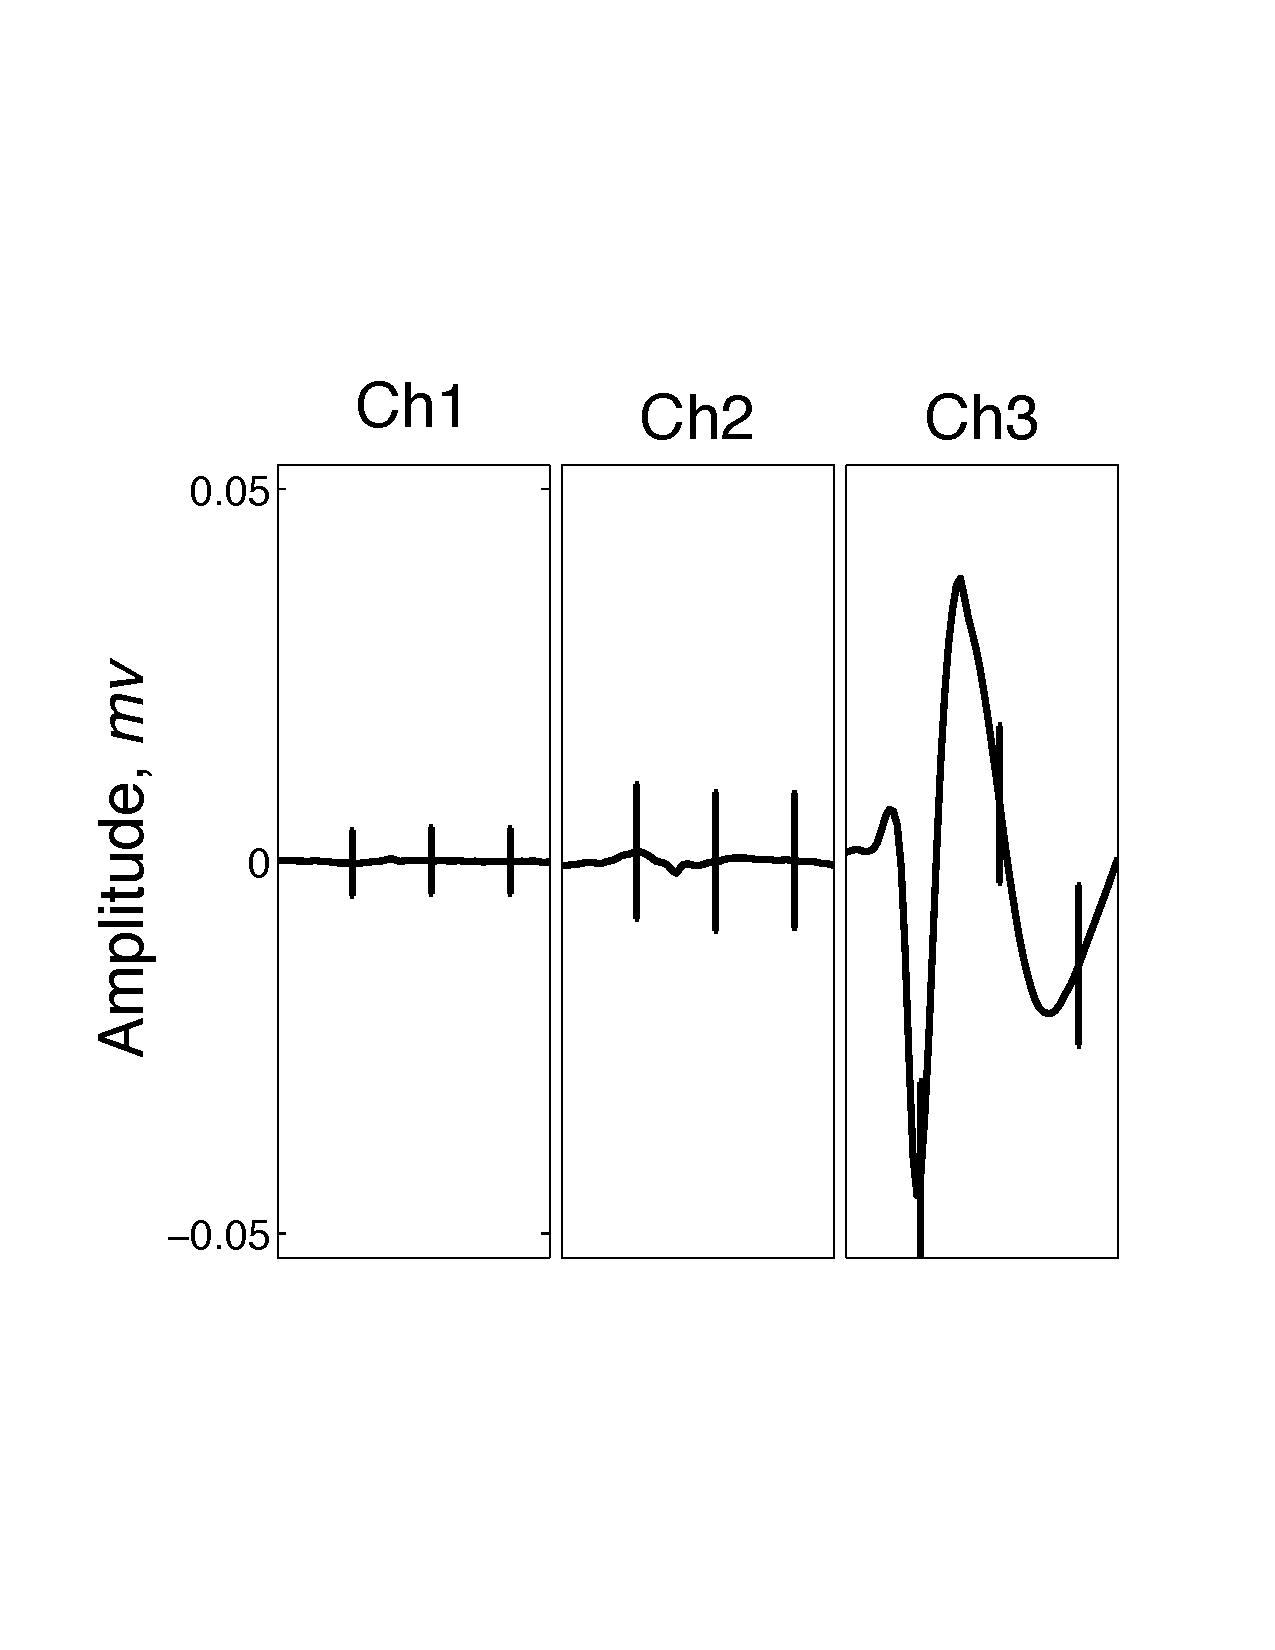
\includegraphics[width=\textwidth]{../figs/3devim/clus2}
% \caption{}
% \label{ex32}
% \end{subfigure}
\begin{subfigure}[b]{.5\textwidth}
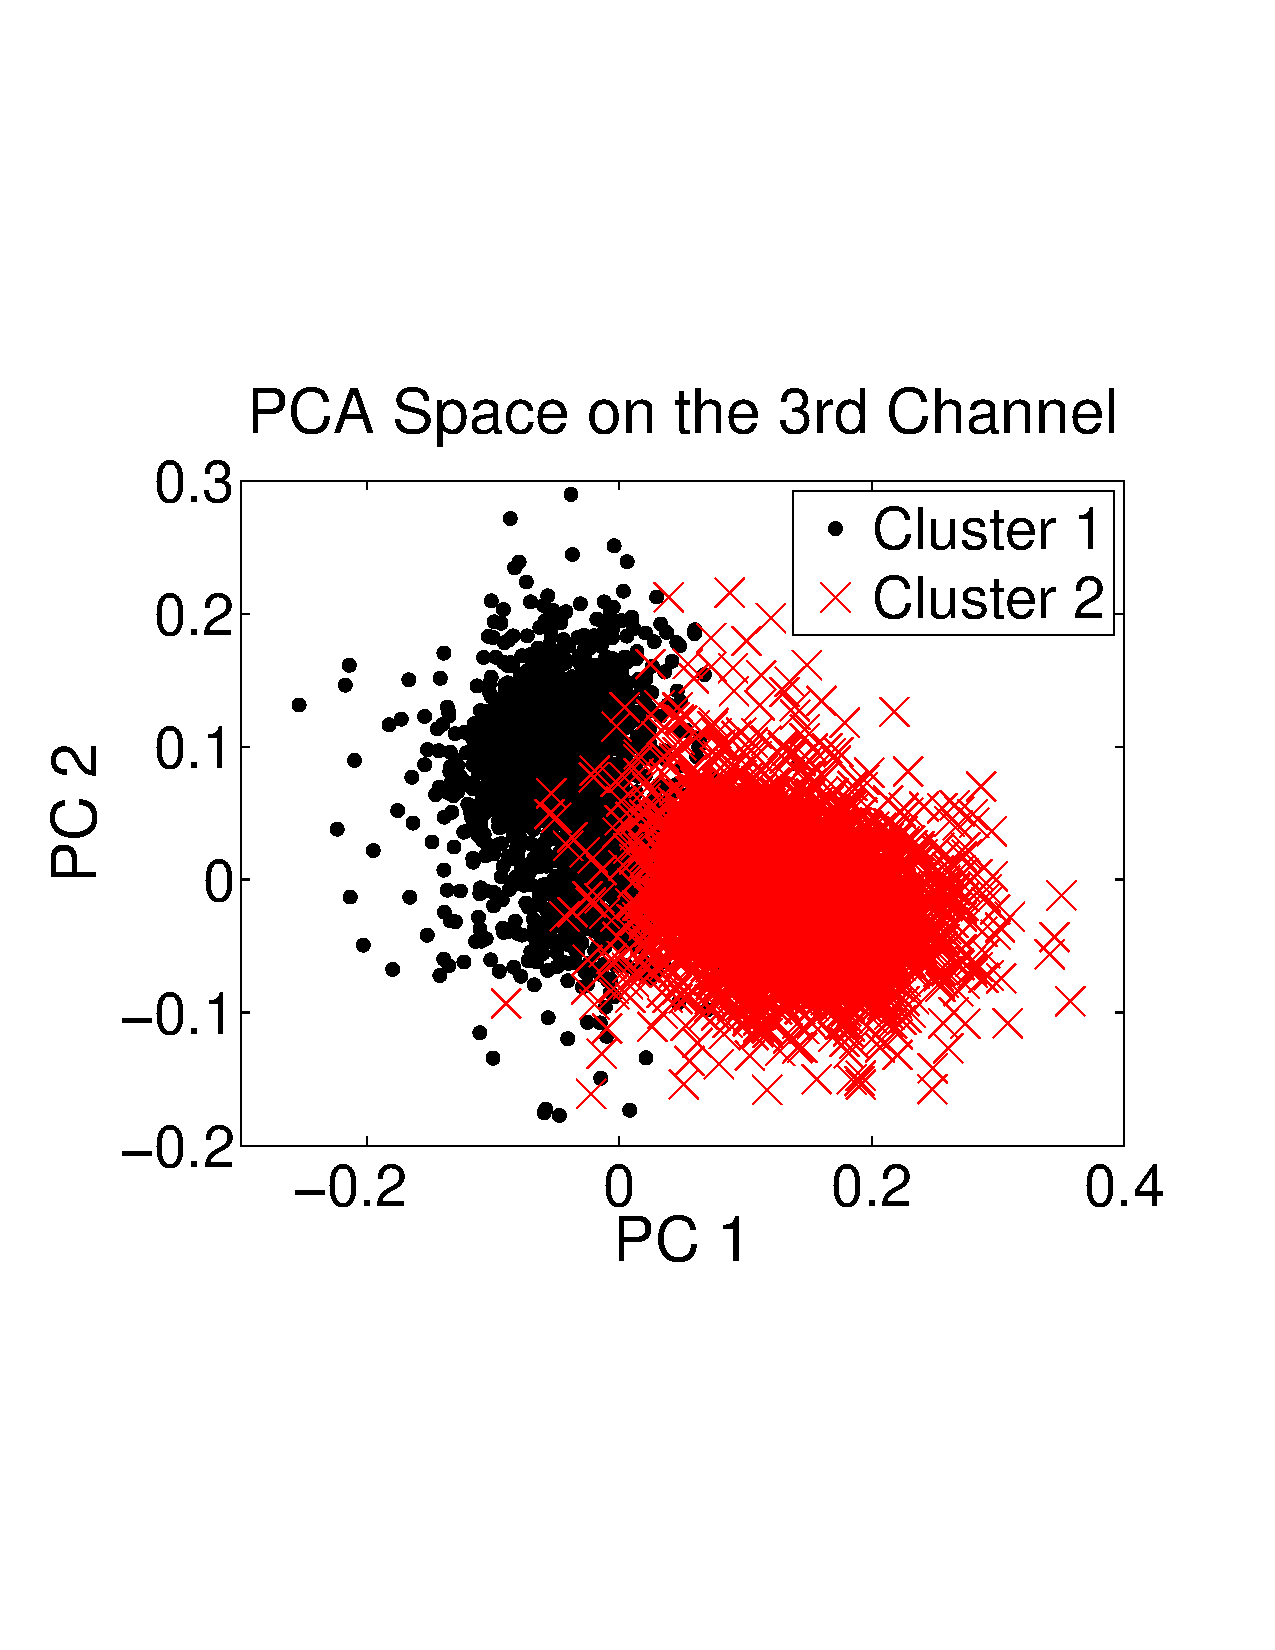
\includegraphics[width=\textwidth]{../figs/new/3chpca}
\caption{}
\label{3chpca}
\end{subfigure}
\caption{
Improving \smug\ by incorporating \emph{multiple} channels.
(a) Three electrode device showing local proximity of electrodes with channel indexes in large, red numbers. 
% (b,c) Top 2 most prevalent waveforms.  Each waveform shape is 2ms long.   Note in (a) we have a waveform that appears on both channel 2 and channel 3, whereas in (b) the waveform only appears in channel 3.  If only channel 3 was used, it would be difficult to separate the waveform in (a) and (b), as is demonstrated in Fig.\ 
(b) The representation of detected spikes on the 3rd channel in PCA space. This cluster does not seem separable here.
}
\end{figure}
\end{center}


% 
% \begin{figure}[htbp]
% 	\centering
% 		% 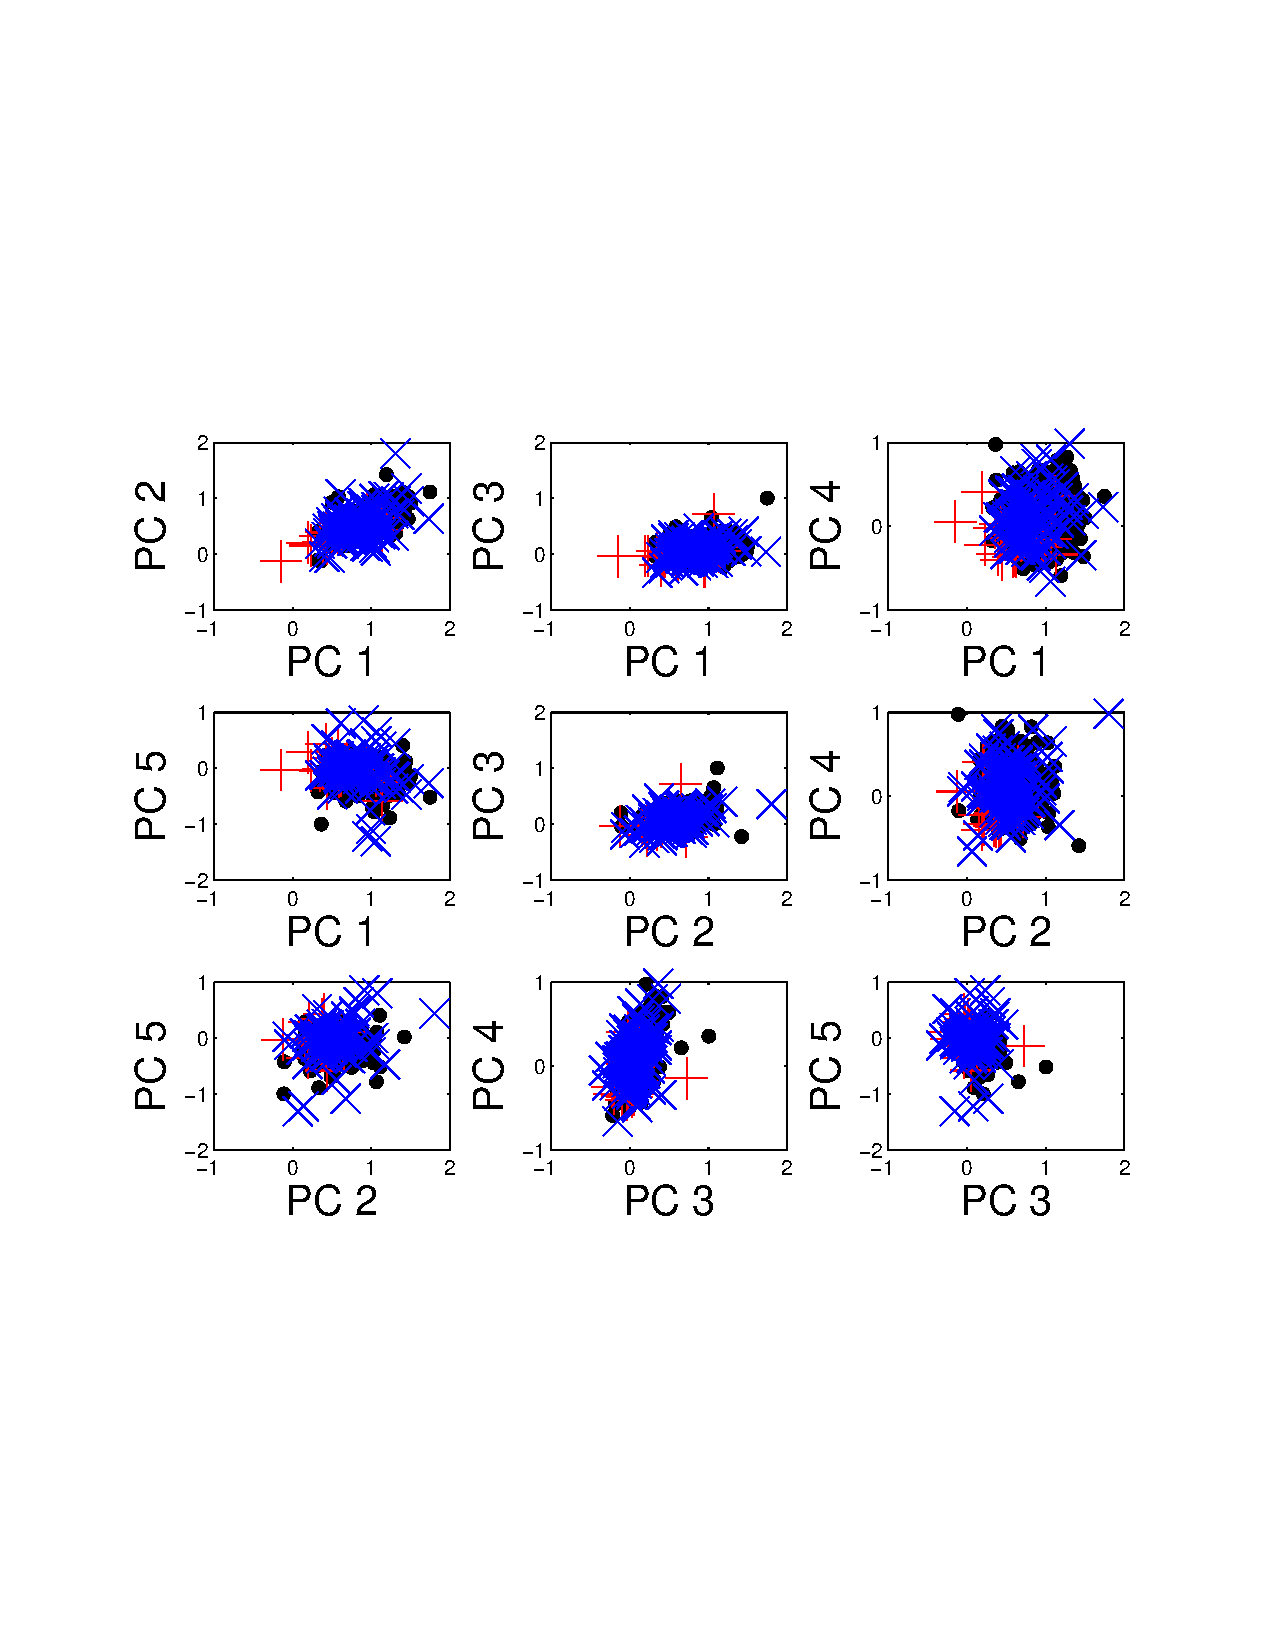
\includegraphics[height=3in]{../figs/new/pairs.pdf}
% 	\caption{(a) intracellular waveform shape over time (b) and in PC space.}
% 	\label{fig:pairs}
% \end{figure}



\begin{center}
\begin{figure}
	% 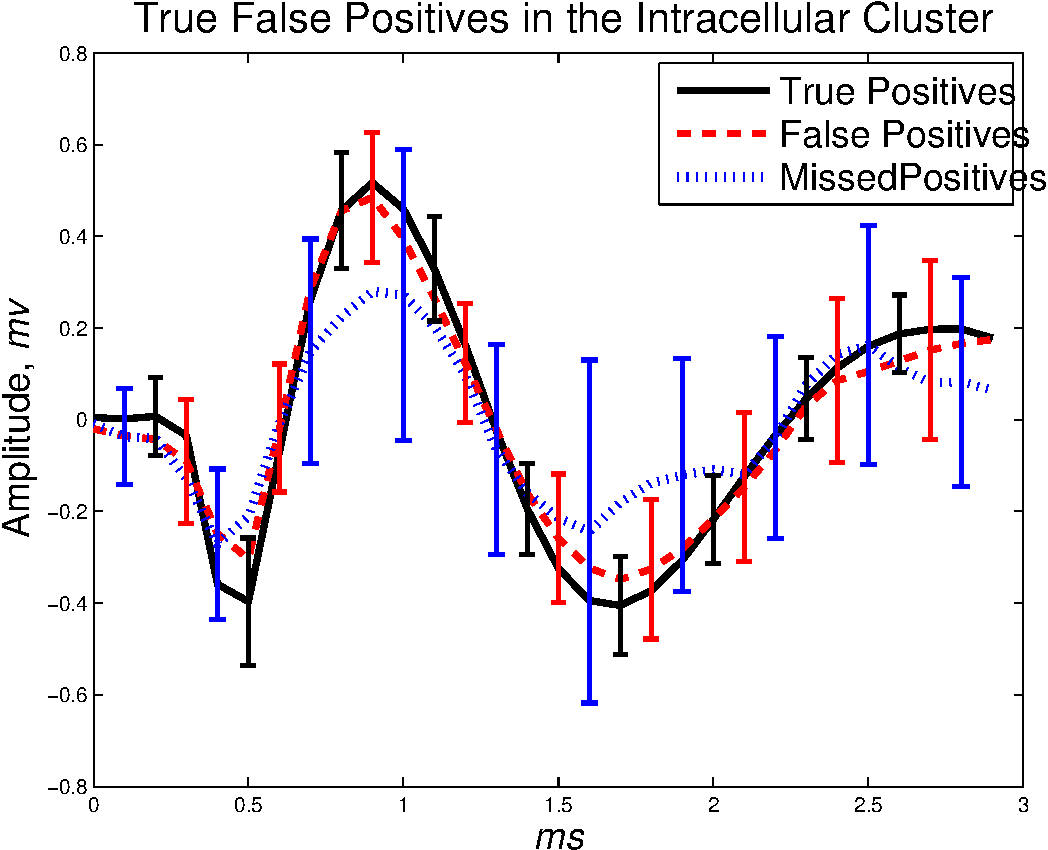
\includegraphics[width=.5\textwidth]{../figs/IntracellularTrueFalsePositivesv2}
	% 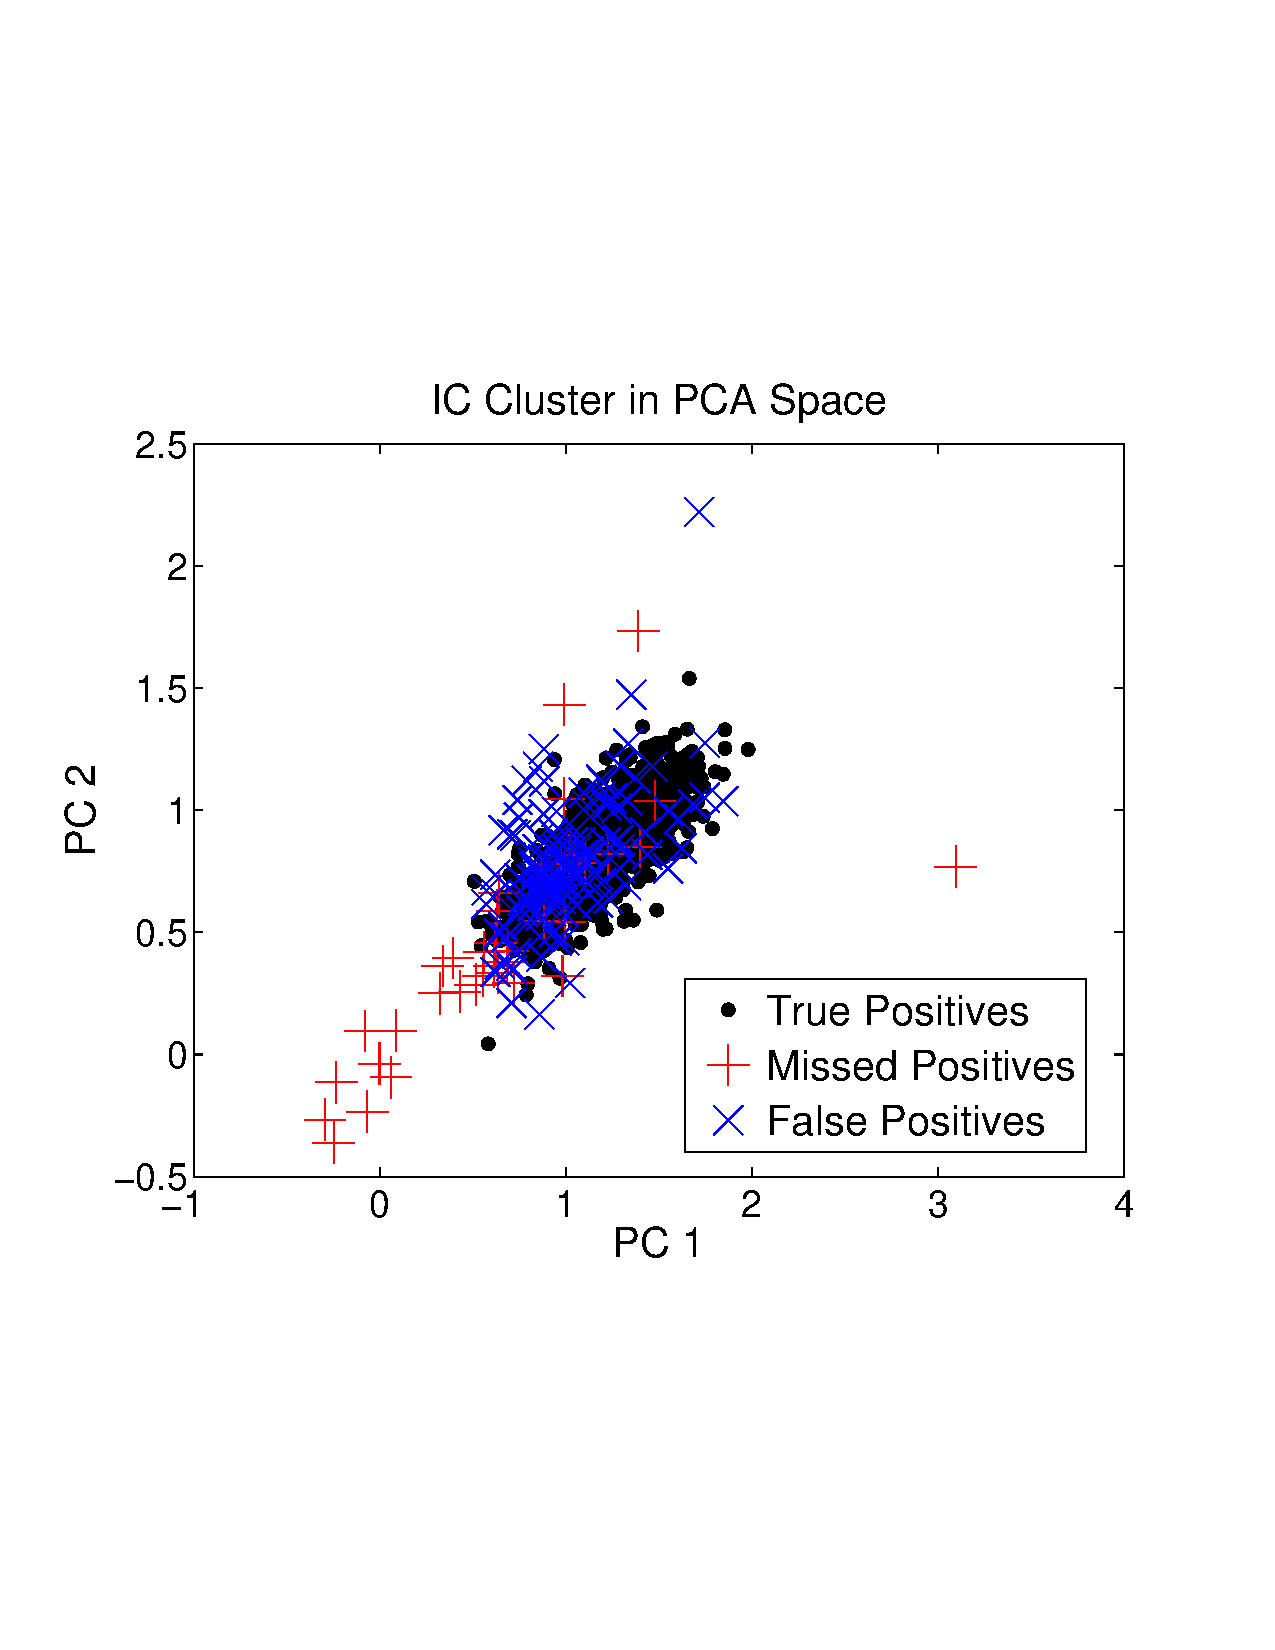
\includegraphics[width=.5\textwidth]{../figs/new/ICclusteroldpca.pdf}
		\begin{subfigure}[b]{.5\textwidth}
	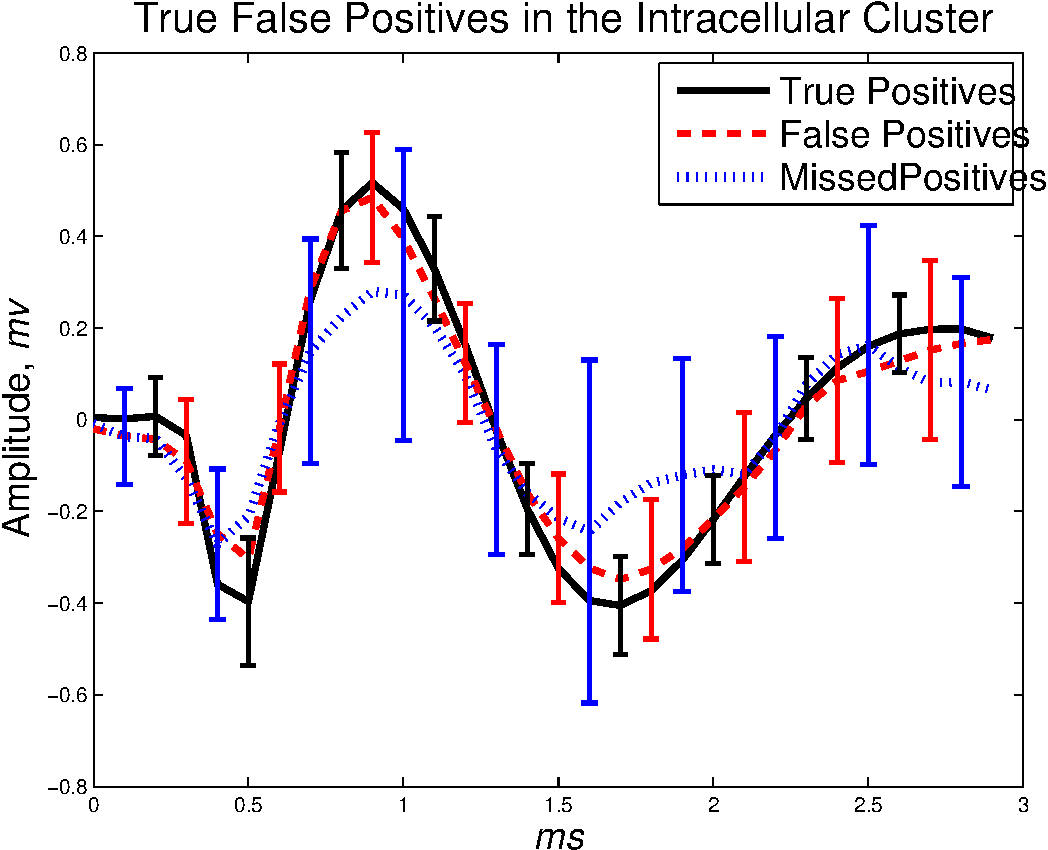
\includegraphics[width=\textwidth]{../figs/IntracellularTrueFalsePositivesv2}
	\caption{}
	\label{truewaveforms}
	\end{subfigure}
\begin{subfigure}[b]{.5\textwidth}
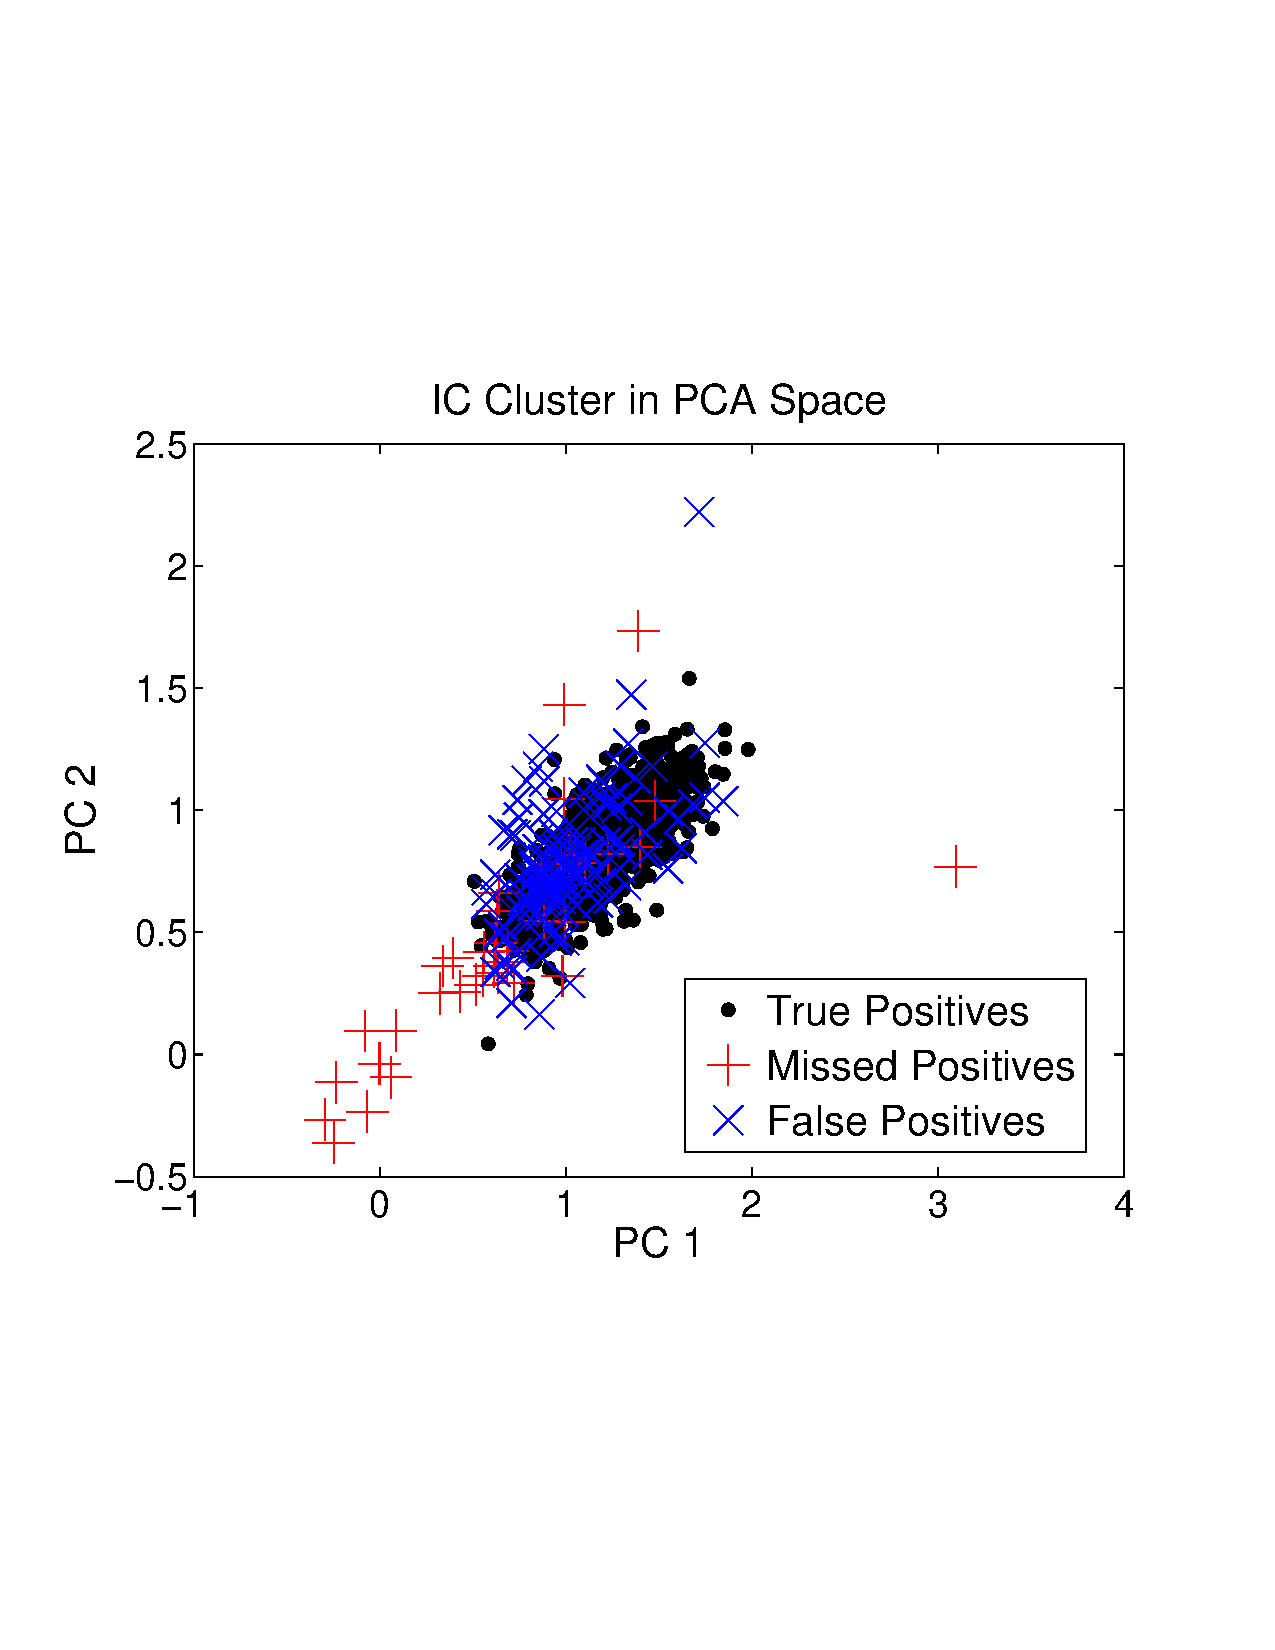
\includegraphics[width=\textwidth]{../figs/new/ICclusteroldpca.pdf}
\caption{}
\label{fig:ICold}
\end{subfigure}
% \begin{subfigure}[b]{.33\textwidth}
% 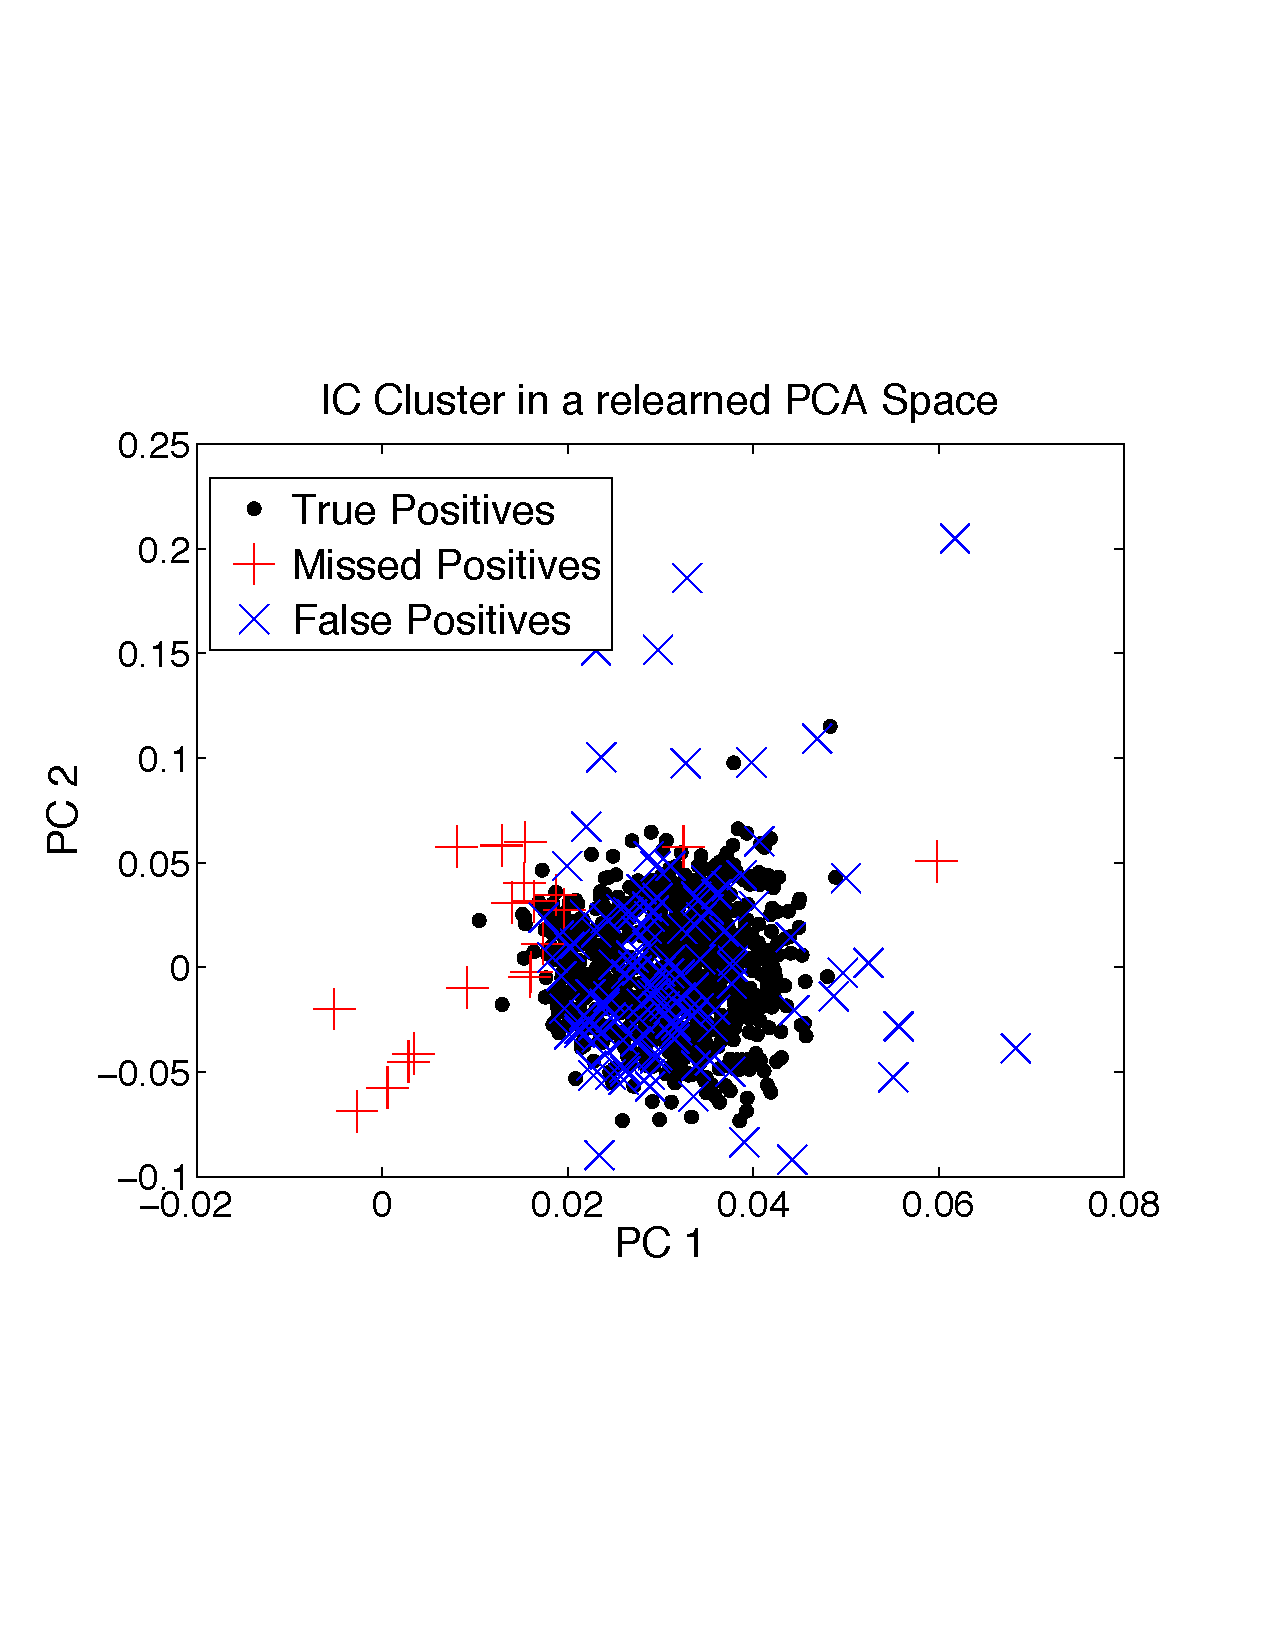
\includegraphics[width=\textwidth]{../figs/new/ICclusternewpca.pdf}
% \caption{}
% \label{fig:ICnew}
% \end{subfigure}
\caption{False and true positive detections have the same first-order statistics, making detection using only these statistics quite difficult.  (a)
 Errorbar plots of the true positives, false positives, and missed positives  in the IC cluster.  While the false positives have slightly more variability, the mean shape for the false positives and the true positives is nearly identical.  The true misses have a significantly lower amplitude as well as high variability. (b) All waveforms from the IC neuron as well as those we estimated from the IC neuron projected onto the first two PC space.} \label{fig:IC-PCA}
\end{figure}
\end{center}

\begin{center}
\begin{figure}[h!]
	% \centering
		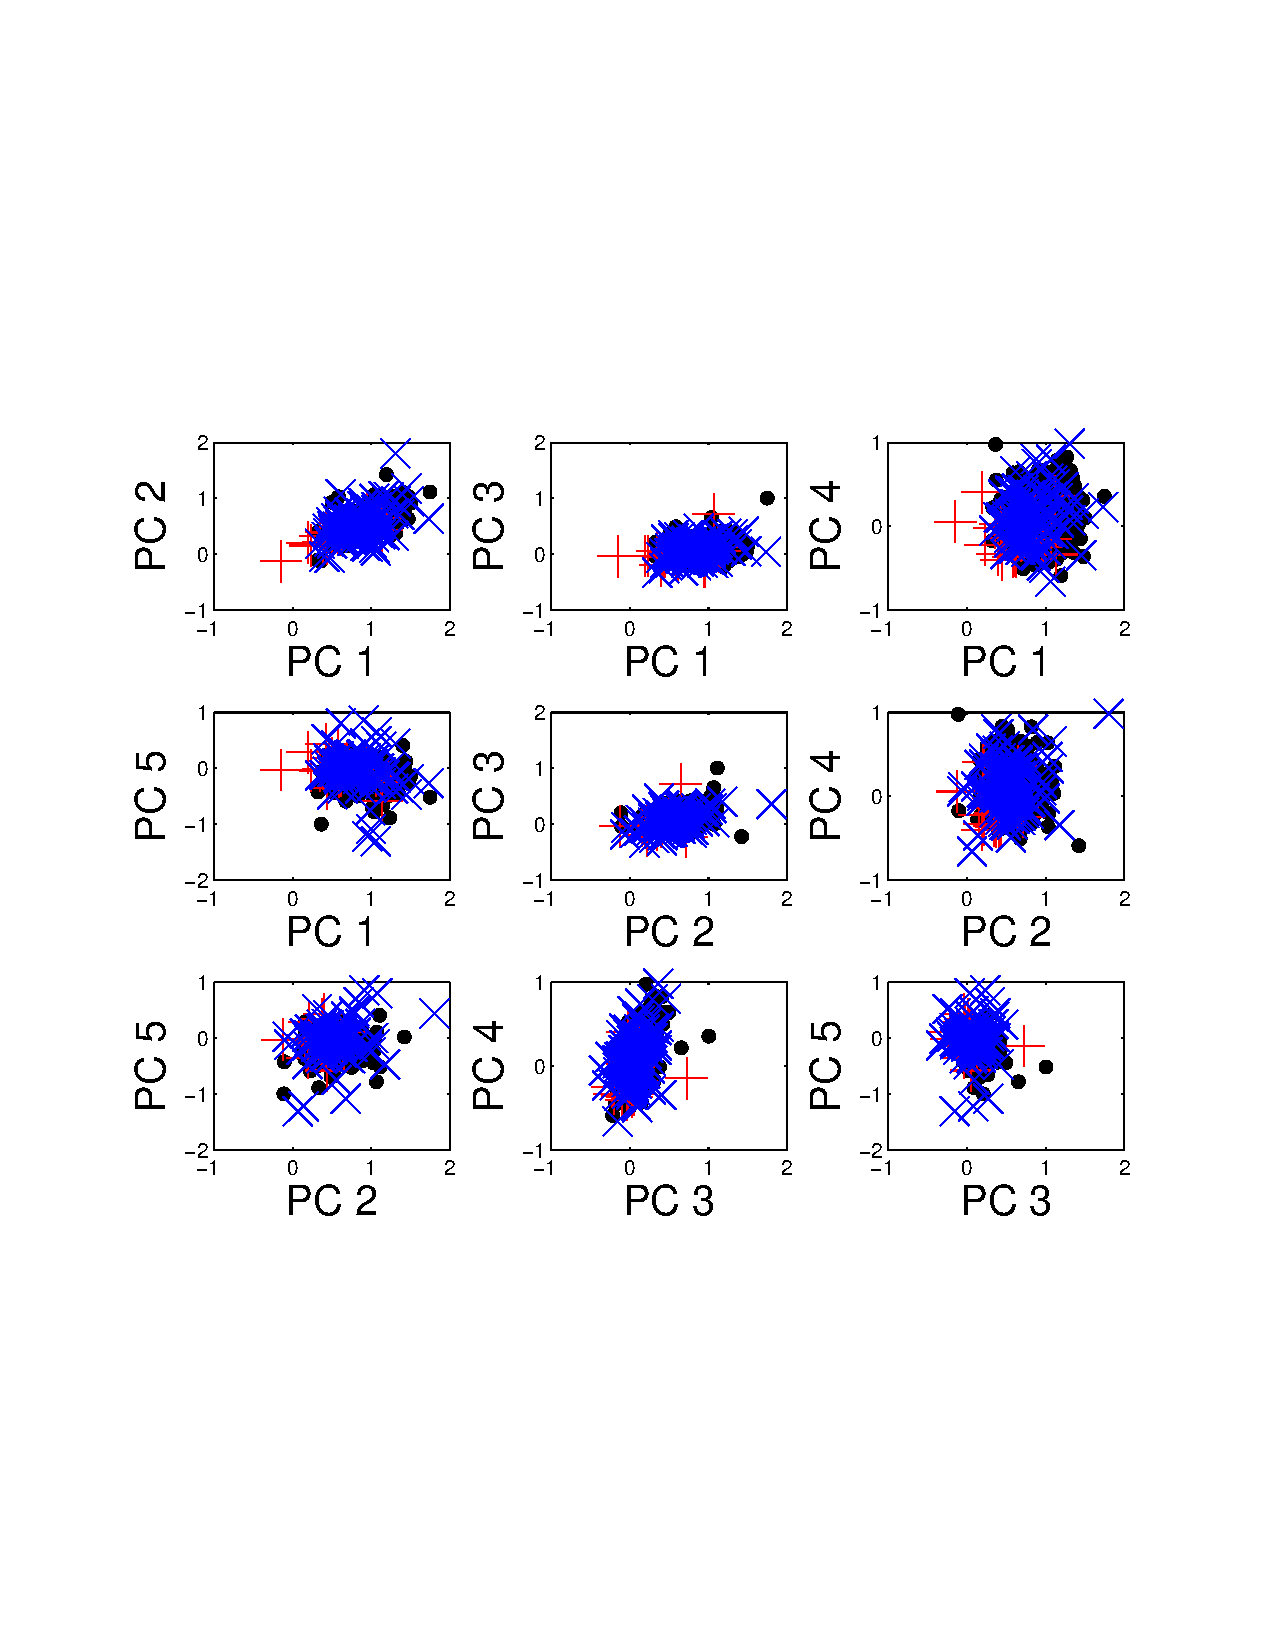
\includegraphics[width=\linewidth]{../figs/new/pairs.pdf}
	\caption{Pairs plot of true positives (black), false positives (blue $\times$'s), and missed positives (red $+$'s).  It does not seem like clustering in this space could yield much improvement. }
	\label{fig:pairs}
\end{figure}
\end{center}

\begin{center}
\begin{figure}
\begin{subfigure}[b]{.12\textwidth}
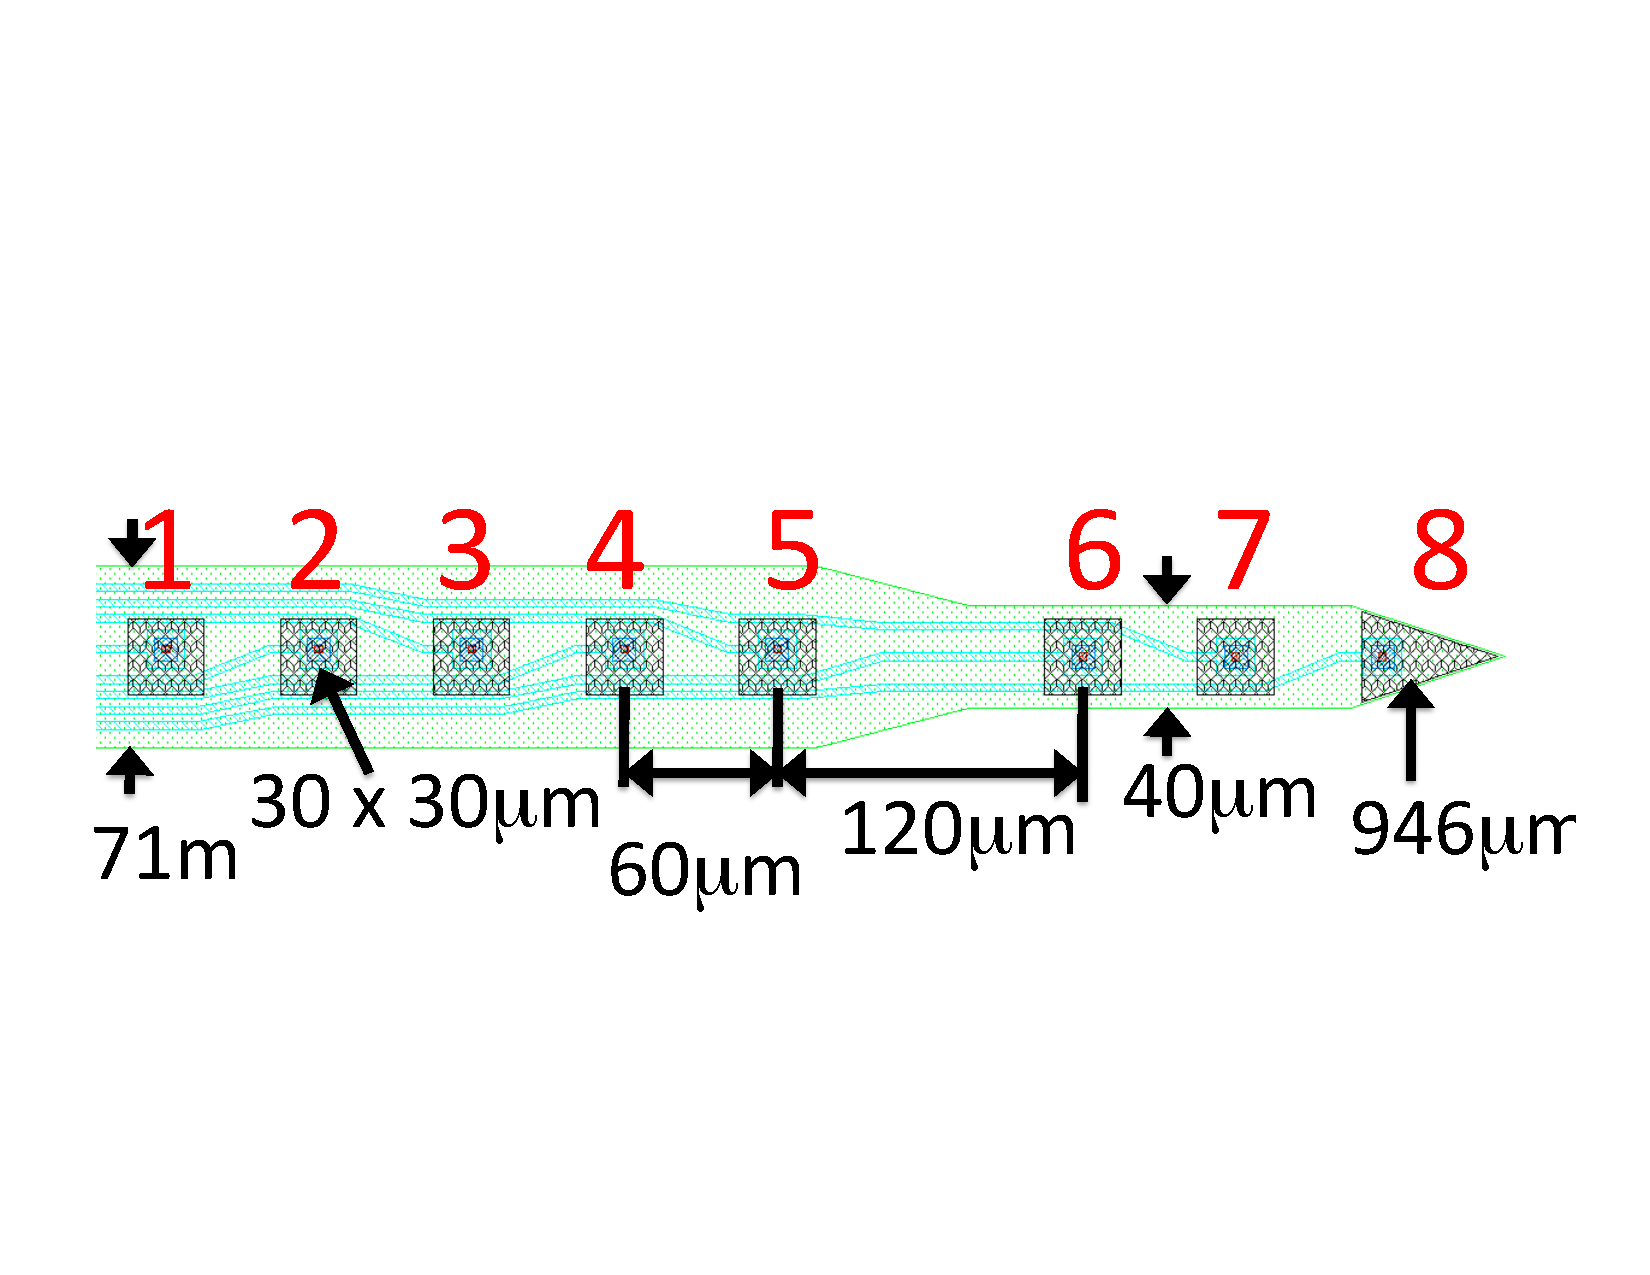
\includegraphics[width=0.8\textwidth]{../figs/8dev}
\caption{}
\label{8dev}
\end{subfigure}
\begin{subfigure}[b]{.28\textwidth}
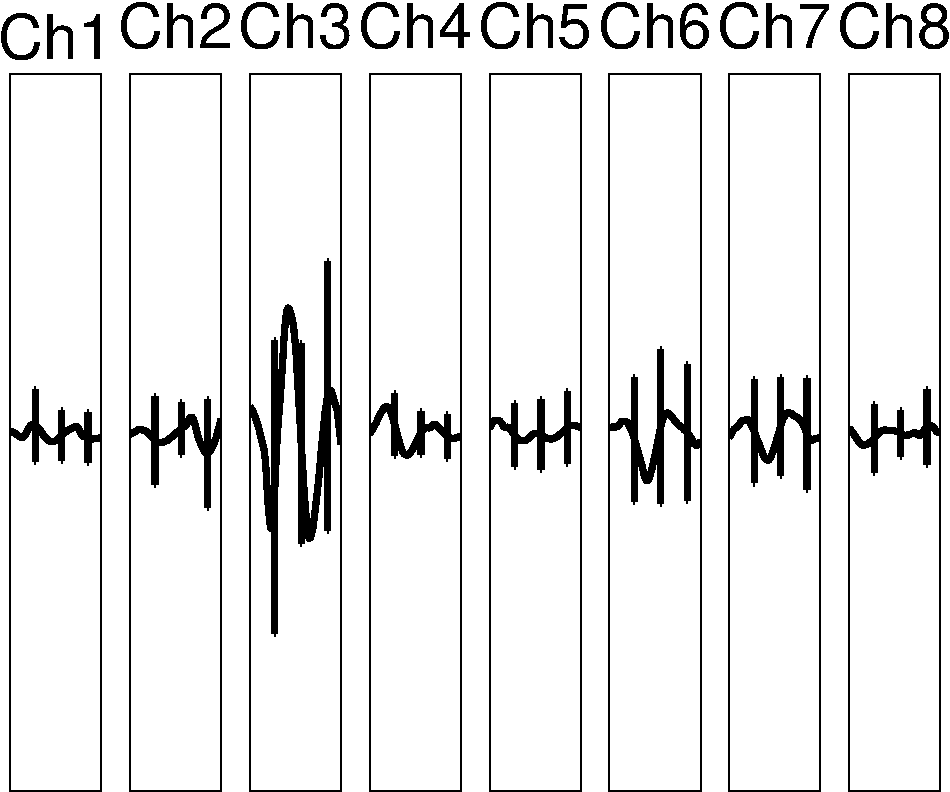
\includegraphics[width=\textwidth]{../figs/8devim/clus3}
\caption{}
\label{ex81}
\end{subfigure}
\begin{subfigure}[b]{.28\textwidth}
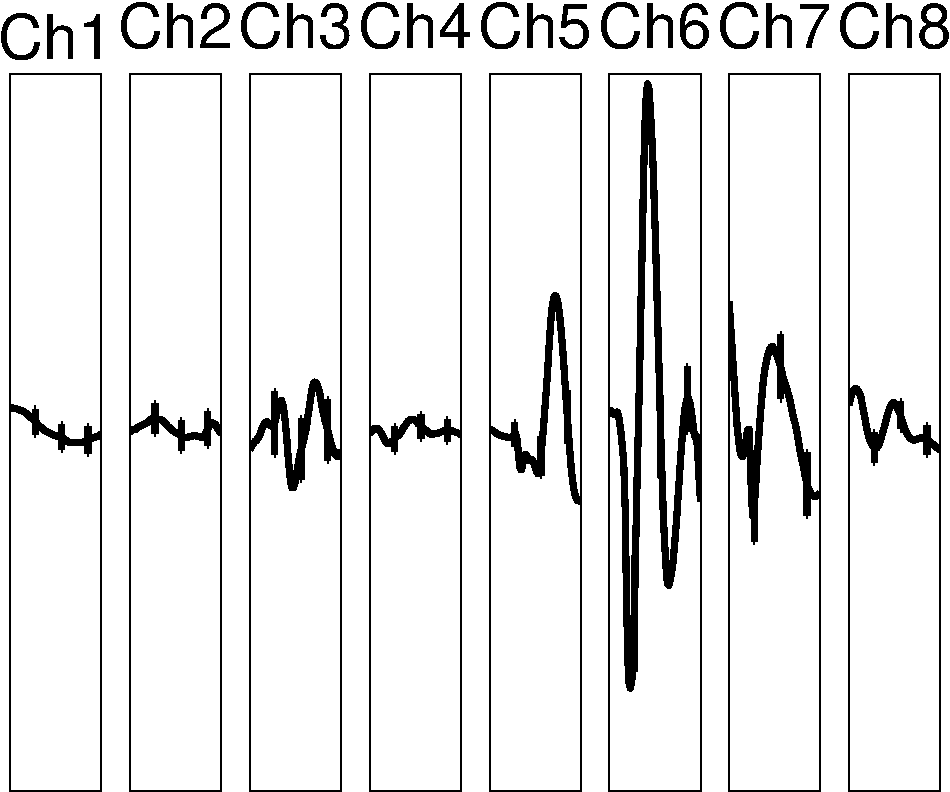
\includegraphics[width=\textwidth]{../figs/8devim/clus9}
\caption{}
\label{ex82}
\end{subfigure}
\begin{subfigure}[b]{.28\textwidth}
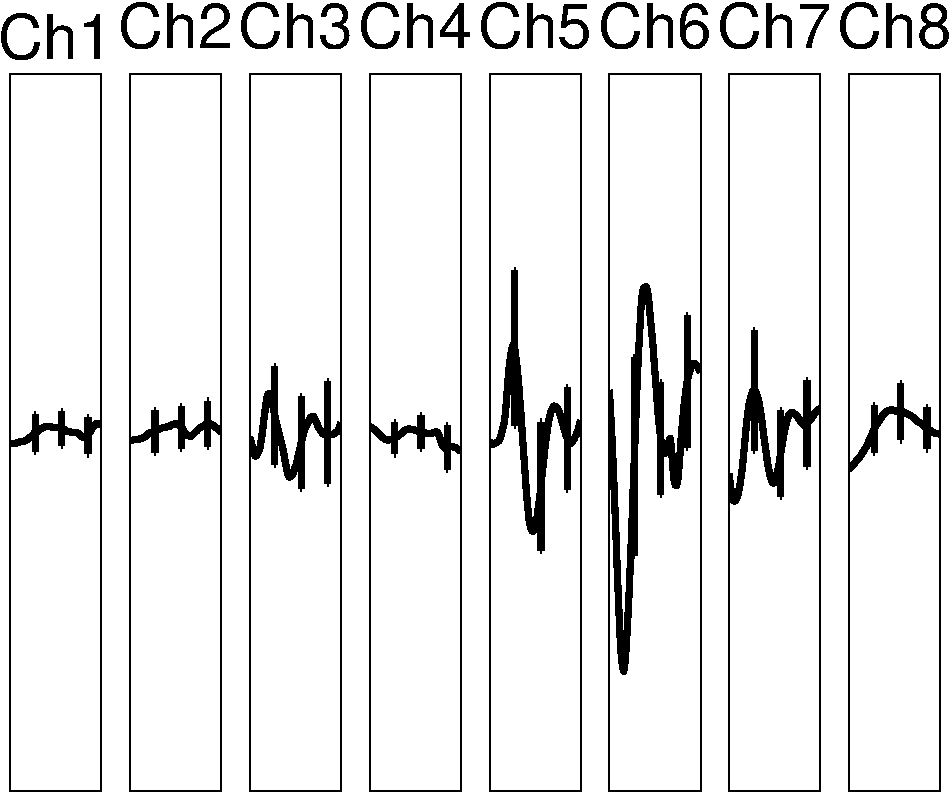
\includegraphics[width=\textwidth]{../figs/8devim/clus6}
\caption{}
\label{ex83}
\end{subfigure}
\caption{
\smug\ multielectrode performance.
(a) 8 electrode device showing local proximity of electrodes with channel indexes in large, red numbers. (b,c,d) Top three most prevalent waveforms.  Each waveform shape is 2 ms long.
} \label{sfig:8}
\end{figure}
\end{center}



\begin{center}
\begin{figure}[h!]
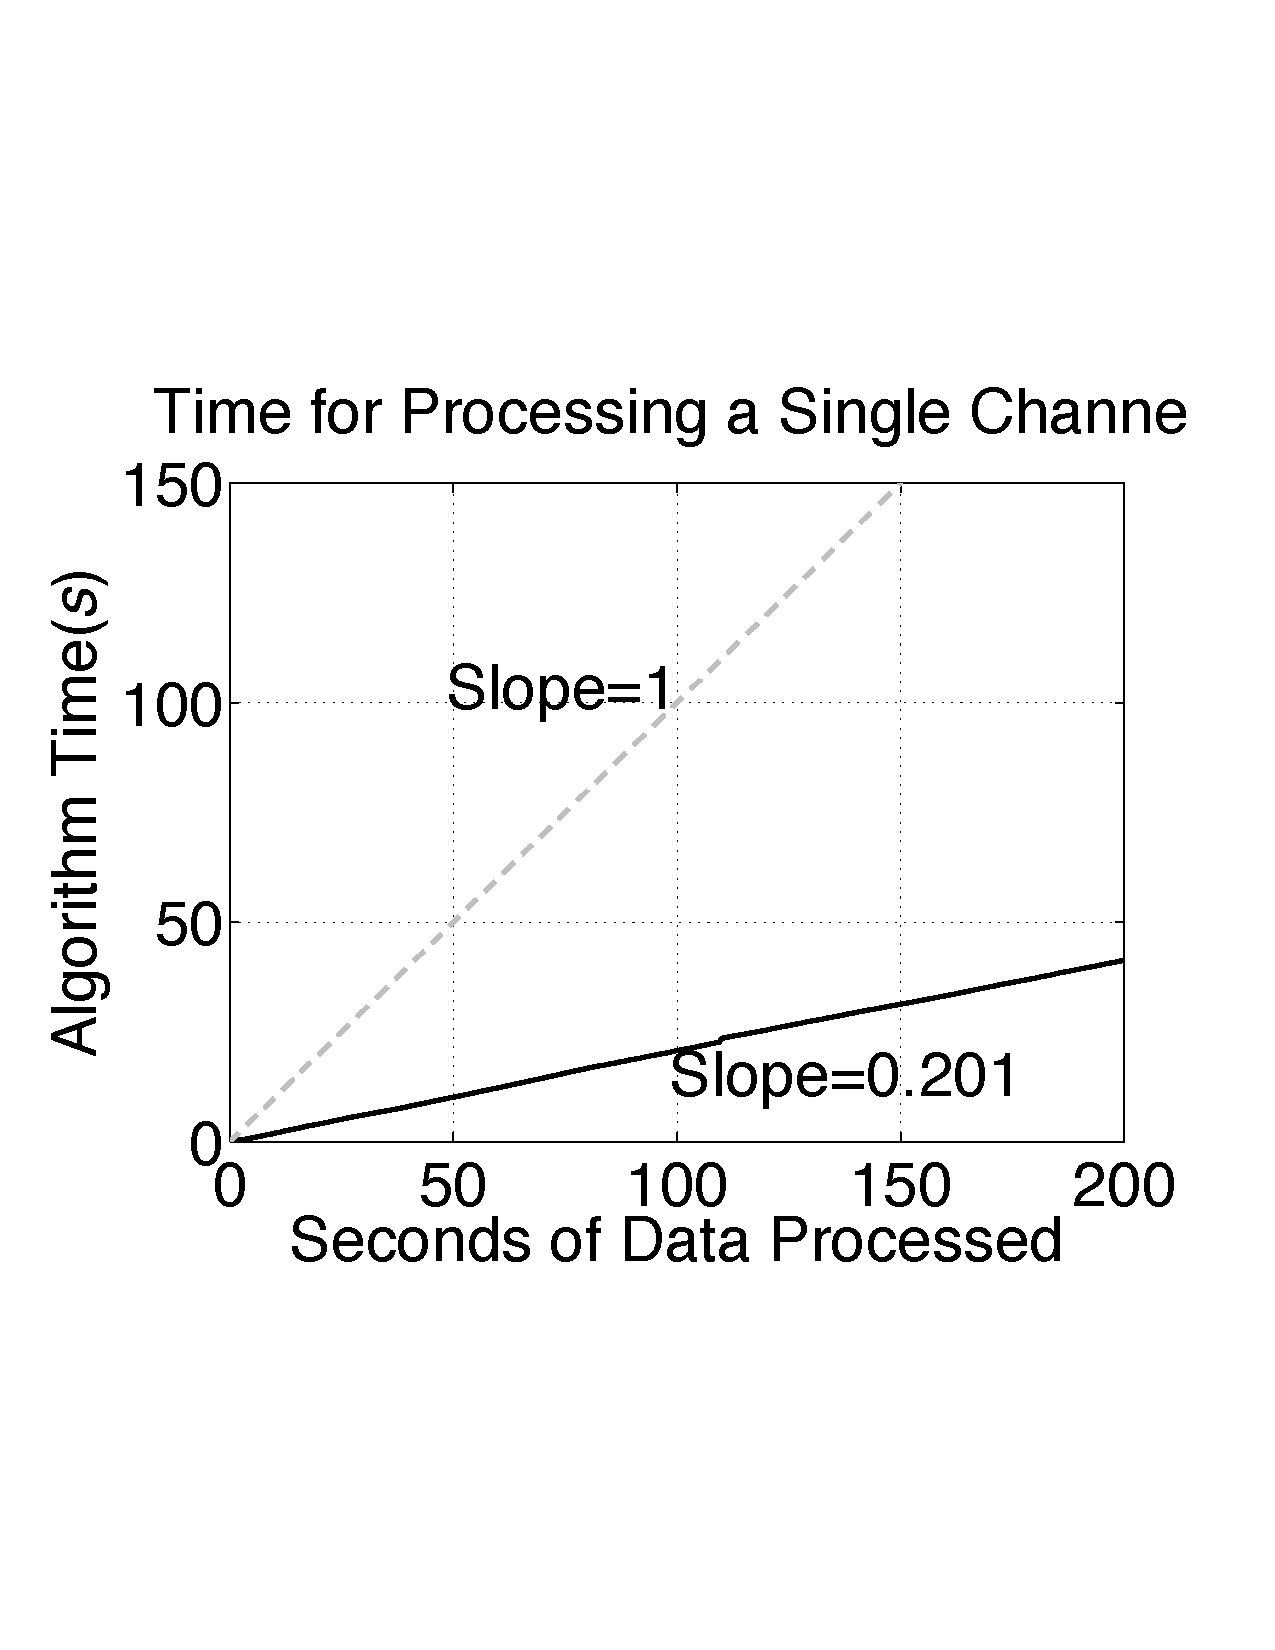
\includegraphics[width=0.5\textwidth]{../figs/new/timingsinglechannel.pdf}
% \begin{subfigure}[b]{.5\textwidth}
% 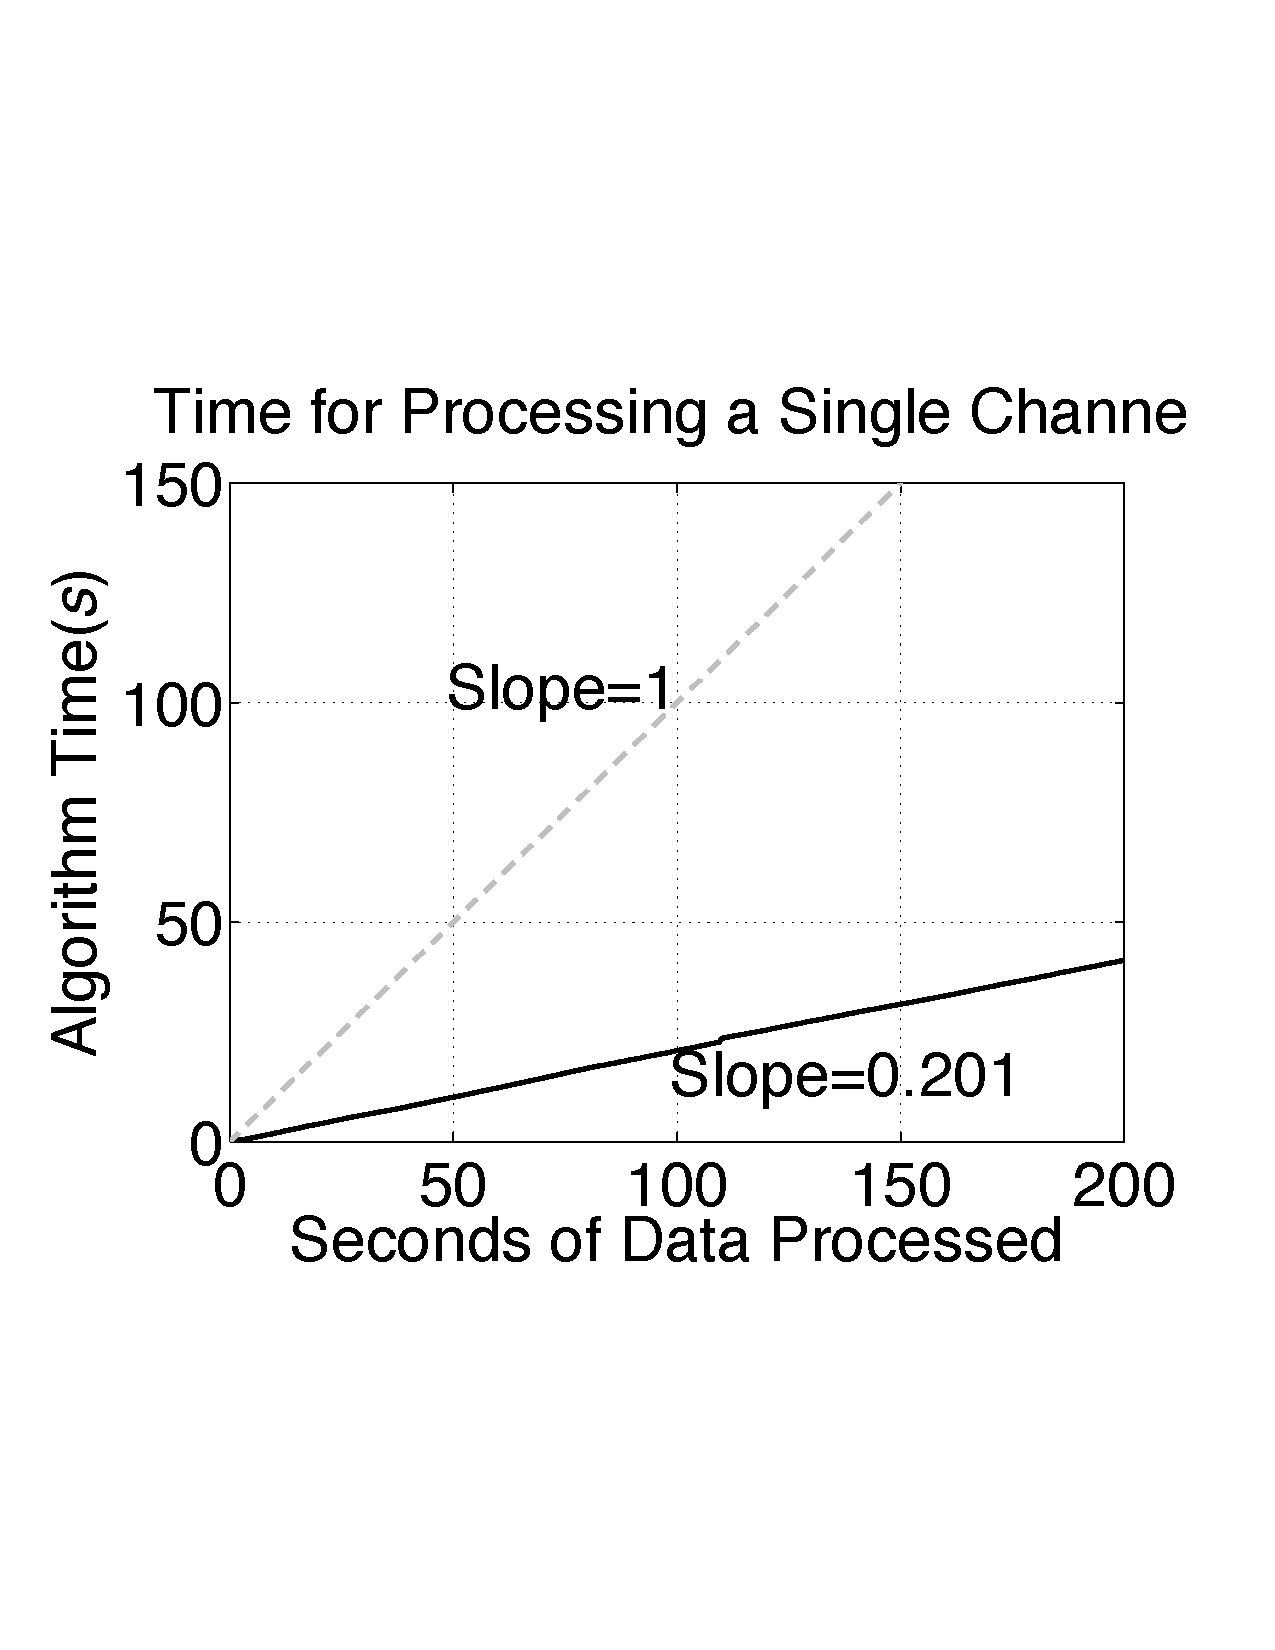
\includegraphics[width=\textwidth]{../figs/new/timingsinglechannel.pdf}
% \caption{}
% \label{fig:ICold}
% \end{subfigure}
% \begin{subfigure}[b]{.5\textwidth}
% % 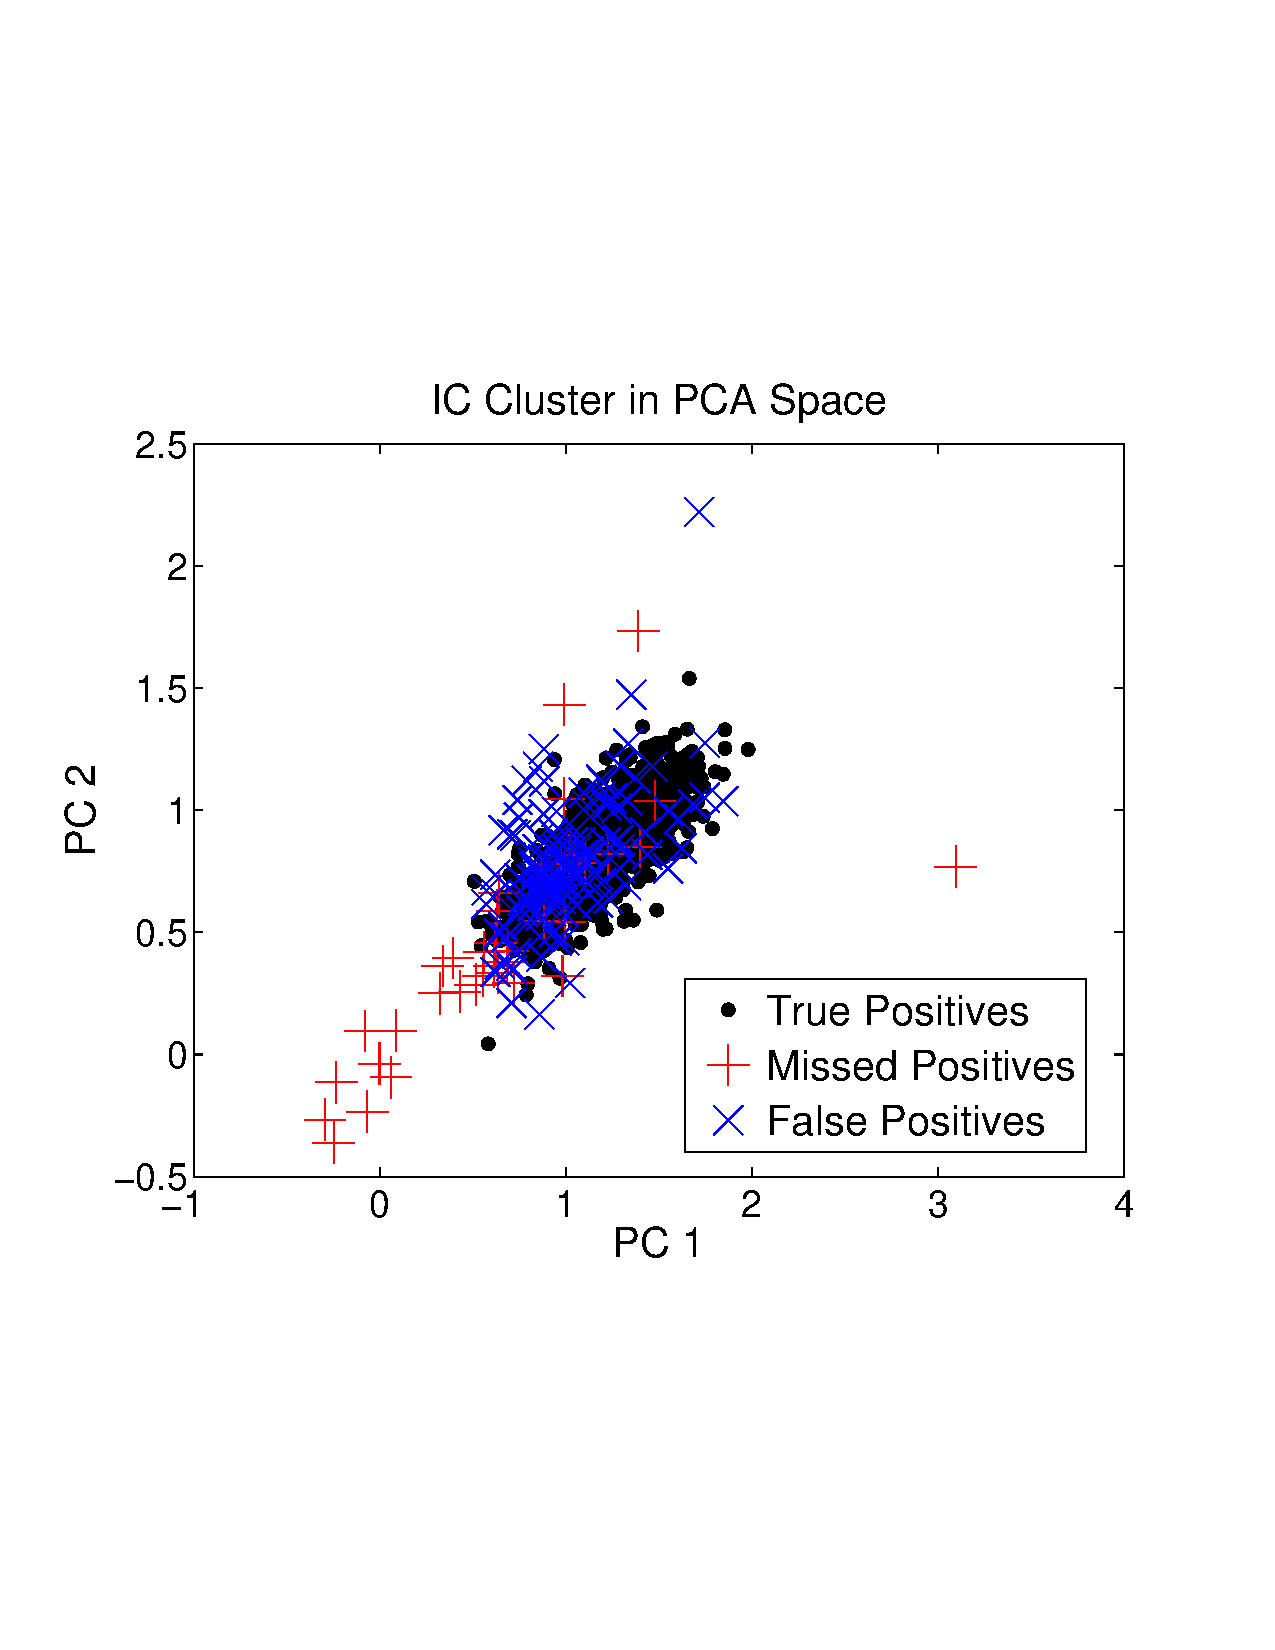
\includegraphics[width=\textwidth]{../figs/new/ICclusteroldpca.pdf}
% \caption{}
% \label{fig:ICold}
% \end{subfigure}
\caption{\smug\ scales linearly with amount of data, with a slope smaller than one, meaning that \smug\ can operate in real-time. } \label{fig:timing}
\end{figure}
\end{center}

